% This is the Reed College LaTeX thesis template. Most of the work
% for the document class was done by Sam Noble (SN), as well as this
% template. Later comments etc. by Ben Salzberg (BTS). Additional
% restructuring and APA support by Jess Youngberg (JY).
% Your comments and suggestions are more than welcome; please email
% them to cus@reed.edu
%
% See https://www.reed.edu/cis/help/LaTeX/index.html for help. There are a
% great bunch of help pages there, with notes on
% getting started, bibtex, etc. Go there and read it if you're not
% already familiar with LaTeX.
%
% Any line that starts with a percent symbol is a comment.
% They won't show up in the document, and are useful for notes
% to yourself and explaining commands.
% Commenting also removes a line from the document;
% very handy for troubleshooting problems. -BTS

% As far as I know, this follows the requirements laid out in
% the 2002-2003 Senior Handbook. Ask a librarian to check the
% document before binding. -SN

%%
%% Preamble
%%
% \documentclass{<something>} must begin each LaTeX document
\documentclass[12pt,twoside]{reedthesis}
% Packages are extensions to the basic LaTeX functions. Whatever you
% want to typeset, there is probably a package out there for it.
% Chemistry (chemtex), screenplays, you name it.
% Check out CTAN to see: https://www.ctan.org/
%%
\usepackage{graphicx,latexsym}
\usepackage{amsmath}
\usepackage{amssymb,amsthm}
\usepackage{longtable,booktabs,setspace}
\usepackage{chemarr} %% Useful for one reaction arrow, useless if you're not a chem major
\usepackage[hyphens]{url}
% Added by CII
\usepackage{hyperref}
\usepackage{lmodern}
\usepackage{float}
\floatplacement{figure}{H}
% Thanks, @Xyv
\usepackage{calc}
% End of CII addition
\usepackage{rotating}

% Next line commented out by CII
%%% \usepackage{natbib}
% Comment out the natbib line above and uncomment the following two lines to use the new
% biblatex-chicago style, for Chicago A. Also make some changes at the end where the
% bibliography is included.
%\usepackage{biblatex-chicago}
%\bibliography{thesis}


% Added by CII (Thanks, Hadley!)
% Use ref for internal links
\renewcommand{\hyperref}[2][???]{\autoref{#1}}
\def\chapterautorefname{Chapter}
\def\sectionautorefname{Section}
\def\subsectionautorefname{Subsection}
% End of CII addition

% Added by CII
\usepackage{caption}
\captionsetup{width=5in}
% End of CII addition

% \usepackage{times} % other fonts are available like times, bookman, charter, palatino

% Syntax highlighting #22

% To pass between YAML and LaTeX the dollar signs are added by CII
\title{Pricing Danish Mortgage Bonds using Machine learning for estimation}
\author{Morten Søby Willendrup}
% The month and year that you submit your FINAL draft TO THE LIBRARY (May or December)
\date{Last compiled on 11 februar, 2022}
\division{Faculty of Social Sciences}
\advisor{Stefan Voigt}
\institution{University of Copenhagen}
\degree{Master Thesis}
%If you have two advisors for some reason, you can use the following
% Uncommented out by CII
% End of CII addition

%%% Remember to use the correct department!
\department{Department of economics}
% if you're writing a thesis in an interdisciplinary major,
% uncomment the line below and change the text as appropriate.
% check the Senior Handbook if unsure.
%\thedivisionof{The Established Interdisciplinary Committee for}
% if you want the approval page to say "Approved for the Committee",
% uncomment the next line
%\approvedforthe{Committee}

% Added by CII
%%% Copied from knitr
%% maxwidth is the original width if it's less than linewidth
%% otherwise use linewidth (to make sure the graphics do not exceed the margin)
\makeatletter
\def\maxwidth{ %
  \ifdim\Gin@nat@width>\linewidth
    \linewidth
  \else
    \Gin@nat@width
  \fi
}
\makeatother

% From {rticles}
\newlength{\csllabelwidth}
\setlength{\csllabelwidth}{3em}
\newlength{\cslhangindent}
\setlength{\cslhangindent}{1.5em}
% for Pandoc 2.8 to 2.10.1
\newenvironment{cslreferences}%
  {}%
  {\par}
% For Pandoc 2.11+
% As noted by @mirh [2] is needed instead of [3] for 2.12
\newenvironment{CSLReferences}[2] % #1 hanging-ident, #2 entry spacing
 {% don't indent paragraphs
  \setlength{\parindent}{0pt}
  % turn on hanging indent if param 1 is 1
  \ifodd #1 \everypar{\setlength{\hangindent}{\cslhangindent}}\ignorespaces\fi
  % set entry spacing
  \ifnum #2 > 0
  \setlength{\parskip}{#2\baselineskip}
  \fi
 }%
 {}
\usepackage{calc} % for calculating minipage widths
\newcommand{\CSLBlock}[1]{#1\hfill\break}
\newcommand{\CSLLeftMargin}[1]{\parbox[t]{\csllabelwidth}{#1}}
\newcommand{\CSLRightInline}[1]{\parbox[t]{\linewidth - \csllabelwidth}{#1}}
\newcommand{\CSLIndent}[1]{\hspace{\cslhangindent}#1}

\renewcommand{\contentsname}{Table of Contents}
% End of CII addition

\setlength{\parskip}{0pt}

% Added by CII

\providecommand{\tightlist}{%
  \setlength{\itemsep}{0pt}\setlength{\parskip}{0pt}}

\Acknowledgements{

}

\Dedication{
You can have a dedication here if you wish.
}

\Preface{
This is an example of a thesis setup to use the reed thesis document class
(for LaTeX) and the R bookdown package, in general.
}

\Abstract{
The preface pretty much says it all.

\par

Second paragraph of abstract starts here.
}

	\usepackage{setspace}\onehalfspacing
% End of CII addition
%%
%% End Preamble
%%
%
\begin{document}

% Everything below added by CII
  \maketitle

\frontmatter % this stuff will be roman-numbered
\pagestyle{empty} % this removes page numbers from the frontmatter

  \begin{preface}
    This is an example of a thesis setup to use the reed thesis document class
    (for LaTeX) and the R bookdown package, in general.
  \end{preface}
  \hypersetup{linkcolor=black}
  \setcounter{secnumdepth}{2}
  \setcounter{tocdepth}{2}
  \tableofcontents

  \listoftables

  \listoffigures
  \begin{abstract}
    The preface pretty much says it all.

    \par

    Second paragraph of abstract starts here.
  \end{abstract}
  \begin{dedication}
    You can have a dedication here if you wish.
  \end{dedication}
\mainmatter % here the regular arabic numbering starts
\pagestyle{fancyplain} % turns page numbering back on

\hypertarget{abstract}{%
\chapter*{Abstract}\label{abstract}}
\addcontentsline{toc}{chapter}{Abstract}

Kind words go a long way

\hypertarget{intro}{%
\chapter{Introduction}\label{intro}}

Mortgage bonds have a long history in Denmark, originating from 1797 where a fire in Copenhagen destroyed most of the city in 1795, this event initiated the first mortgage bank (Jensen 2013).

The general idea on how the mortgage system in Denmark has since only seen minor changes thus a source of high stability.

The idea being the system that instead of having a one-to-one relationship between the borrower mortgage loan and the investors mortgage bond.

The Danish mortgage system is structured such that borrowers have their loans pooled, to which bonds is issue.

When an investor buys a bond issued from the pool, this is equivalent to buying a share of the pooled loans, in which the investor is entitled to receive interest payments and repayment proportional to the invested amount.

What makes the Danish mortgage system distinguishable is the balance principle. This principle ensures an almost perfect match between the interest and repayments paid and received by the borrowers and investors respectively.

Figure \ref{fig:bondCashFlow} illustrates the cash flows that occurs between the borrow, the mortgage bank and the investor. When a loan is granted to a borrower, the mortgage bank issues a bond in the primary market accordingly. The investor then buys the bonds and the process from the trades go to the borrower thus giving the borrower liquidity to purchase the dwelling on which the loan is based.

The borrower will pay interest, repayments and fees known as the so-called ``bidragssats'' to the mortgage bank, who facilitate that the interest and repayments are passed through to the investor and thereby keeping the fees to cover their costs of issuing the bonds and the adherent risk associated with the issuance of bonds, since the issuing mortgage bank takes on the risk opposed to the borrower.

The credit risk of the borrower is towards the mortgage bank, and since the housing is used at collateral in the agreement the credit risk is lowered in the viewpoint of the mortgage bank.

The default risk held by the investor is even more reduced since the mortgage bank has go into default before the investor will be exposed to a credit event. In a potential credit event of the mortgage bank, the investors will have the right to the cover pool, which is separate legal structure ensuring that the bond investors in a credit event does not have share to their claim towards the mortgage bank along with other creditors.

The cover pool will consist of collateral in terms of the claims against the borrows as well as additional securities posed by the mortgage bank to protect the investor from losses. These securities constitute what is known as overcollateralization and should be of very high credit quality.

Since modelling will be performed from the investors point of view, and the default risk held by the investor has been brought to a minimum, the paper will not include default risk in our model.
\begin{figure}

{\centering 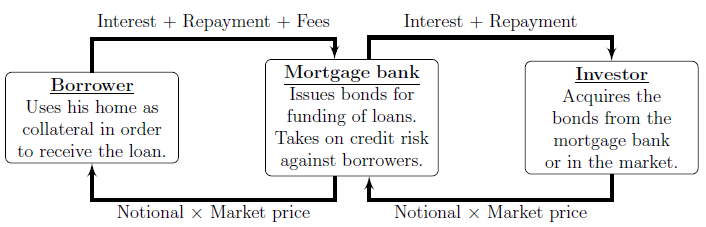
\includegraphics[width=1\linewidth]{figure/bond_cash_flow_illustration_23012022} 

}

\caption{Simplified illustration of the relationships and payment streams between the homeowner, the mortgage bank and the investor in the Danish mortgage system.}\label{fig:bondCashFlow}
\end{figure}
To understand why the Danish mortgage system is of interest is due to impact on
the Danish economy and the significant size of the market, being the largest covered
bond market in Europe (ECBC 2021), where in December 2021 the Danish mortgage market amounted to DKK 3,177 billions.

According to the Danish central bank, Nationalization, the foreign ownership of Danish Mortgage bonds totalled DKK 802 billions as of Dec 2021 or equivalent to 24\% of the total amount outstanding in the Danish mortgage system.

THe market for Danish mortgage bonds consits mainly of fixed coupon callable bonds, adjustable rate mortgage bonds and capped floating rate bonds.

The focus of this thesis will be on the fixed income coupon callable bonds due it being the most complex of the aforementioned.,

In order to understand the different aspects of a callable bond, we will first have to introduce the term structure theory and build a framework for descrying the behaviour of the yield curve. This in done in \ref{theory}

\hypertarget{the-danish-mortgage-market}{%
\chapter{The Danish Mortgage Market}\label{the-danish-mortgage-market}}

Being one of the oldest and most stable bond markets in the world, the Danish Bond market has it's root all the way back to 1797 where the first mortgage bank Kreditkassen for Husejere i Kjøbenhavn was established to help rebuild Copenhagen after the devastating fire of 1795 where a quarter of the city was lost to the fire.

The objective of stabilibty can also be seen in the resistance of the Danish Mortgage Market to economic crises, as the Danish economy has gone through several crises the past 50 years.
\begin{itemize}
\tightlist
\item
  The two oil crises of the 1970's
\item
  The 1986 austerity package and the 1987 tax reform
\item
  The Dot-com bubble in 2000
\item
  The financial crises
\end{itemize}
Arguable each crises has had an effect on the mortgage system differently and have even caused substitutional losses to the mortgage banks. However the losses have never affected the investors, as not one Danish Mortgage bondholder has lost the investment or even part of it. Moreover, the market stayed active and liquid under the financial crisis as evidenced by (Dick-Nielsen, Feldhütter, and Lando 2012; Gundersen, Hesselberg, and Hove 2011), where both find that the Danish Mortgage Bonds were as liqui as the Danish Government bonds during years from 2008 to 2009.

\hypertarget{types-of-mortgage-bonds}{%
\section{Types of mortgage bonds}\label{types-of-mortgage-bonds}}

The Danish mortgage market mainly consists of the following types of mortgage bonds
\begin{itemize}
\item
  ARMs - Adjustable Rate Mortgage Securities. which are subject to refinancing until the longer-term underlying loan has matured. The maturities match the fixed-rate period of the underlying loan, and are mainly 1 to 5 yers and the bond type is bullet
\item
  Floating-rate note - Variable-rate annuities with redemptions matching the underlying loans. The maturites mainly range from 1 to 5 years.
\item
  Capped floater - Variable-rate annuities with redemptions not matching the underlying loans. The maturites are mainly from 5 to 30 years
\item
  Callable bonds - Fixed rate callable annuities, where payments and redemptions match the underlying loan. The maturities are mainly 15, 20 or 30 years.
\end{itemize}
All 4 types of mortgage bonds have underlying loans where maturires of up to 30 years are available. Furthermore, most loans can be offered with an interest only(IO) period up to 30 years. If the IO option is chosen, the loan must be repaid as an bullet bond at maturity, otherwise if a IO period of 10 years is chosen, the loan must be repaid as an annuity profile for the remaining lifetime of the loan i.e.~20 years. In recent years the amount of loans with interest only option has declined and as of December 2021, interest only loans accounts for 43.5 \%\footnote{Nationalbanken Statistics - DNRUDDKI} of the loans to Danish house-holds.

\hypertarget{the-danish-mortgage-model}{%
\section{The Danish mortgage model}\label{the-danish-mortgage-model}}

The Danish mortgage model is based upon a stable and transparent system, with several advantages and unique features. Since mortgage banks does not function as commercial banks, and only able to fund loans through the sale of bonds which limits the risk of the mortgage banks Hence, the mortgage bank protects the investor from borrower defaulting. The mortgage bank secures the issued bond by using the cover pool which consist of collateral in terms of the claims against the borrows as well as additional securities posed by the mortgage bank to protect the investor from losses. These securities constitute what is known as overcollateralization and should be of very high credit quality.

\hypertarget{balance}{%
\section{Balance principle}\label{balance}}

The Balance principle entails that for every loan made by the mortgage bank, a new bond is issued with matching cash-flow properties. This eliminates mismatch in cash-flows and refinancing risk for the mortgage bank, which also secures payments to the bondholder. In the Danish mortgage system the mortgage bank functions as an intermediary between the investor and the borrower. Mortgage banks funds loans on a current basis, meaning that hte bond must be sold before the loan can be given. This also entails that the market price of the bond determines the loan rate. THe loan is therefore equal to the investment, which passes through the mortgage bank. Repayment and interest from the borrower to investor also passed through them mortgage bank, however the mortgage bank changes the borrower a margin though the lifetime of the loan, which is a percentage of the debt outstanding.

Since mortgage banks is only an intermediary it is not affected by changes in the floating rate, as it passes repayments and interest through to the investor. The drawback for the mortgage bank is that it endures the credit risk in the event of a default of the borrower, as it still has to make repayment and interest to the bond holder. This however protects the investor as the credit risk is removed, but is also a great incentive for the mortgage bank to put an emphasis on the due diligence process when issuing loans and adds to the stability of the system. Part of the due diligence is not only the valuing the property when making a credit assessment of a potential borrower, but also assessing the borrower's current economic situation including income and wealth based on legislation that dictates eligibility for granting and funding loans.

\hypertarget{delivery-and-prepayment}{%
\section{Delivery and prepayment}\label{delivery-and-prepayment}}

A central unique feature of the Danish mortgage model is the delivery option which means that the borrower always has the possibility of buying the underlying bond in the market, and delivering it back to the mortgage bank, which then cancels the loan. This is unique way for the borrower to reduce the notional amount of the loan if interest rate rises, and the related bond price falls. It is also a hedging effect on the expected drop in house prices that follows increasing interest rates as the two effect offset each other. This has no effect on the investor in terms of payments made from the investors to the bondholders.

Callables bonds also have a prepayment option( embedded call-option). The prepayment option gives the borrower the opportunity to repay the loan at pari (100) at every quarter throughout the lifetime of the loan.

Capped floaters have a similar prepayment option, however the prices depends on the contract is typically 105. This is favorable when the current available coupon rate is below the coupon rate on the mortgage.

The prepayment on Danish callables and capped floaters are more difficult to price than corresponding bond without the prepayment option and come with an additional option and come with an additional prepayment risk for the investor, this is however compensated with a higher interest rate.

The prepayment risk arises from the option to prepay the loan at pari, which exposes the investor to the risk of not being able to reinvest at the same conditions. The rational scenarios for prepayment are depicted in figure \ref{fig:prepayment}
\begin{figure}

{\centering 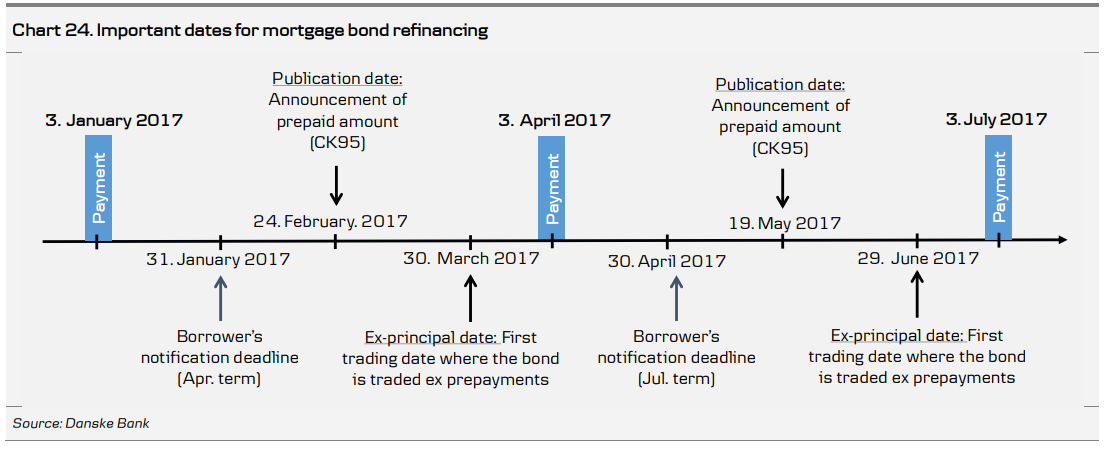
\includegraphics[width=1\linewidth]{figure/Prepayment_notice_dates} 

}

\caption{Pricing curve of Callabalbe Bonds and Non-callable bonds.}(\#fig:important dates)
\end{figure}
When prices are close to par the price of the callable bond is lower than the price of a non-callable bond, i.e.~government bond, as the chance of prepayment increases. However the borrowers are not always rational, which can create opportunities for the active investor, but is also a source of risk for a buy-and-hold strategy.

\hypertarget{callable-annuity-bonds}{%
\section{Callable annuity bonds}\label{callable-annuity-bonds}}

Callable annuity bonds are unique to the Danish covered bond market. Traditionally,
callable annuity bonds were the only type of bonds issued in the Danish covered bond market but the introduction of new products has expanded market diversity. Originally, this type of bond had two payment dates per year but four has been the norm since 1985. Standard payment dates are 1 January, 1 April, 1 July and 1 October. Maturities are primarily 10, 15, 20 or 30 years. Callable annuity bonds are fixed rate bonds with an embedded call option. The embedded call option enables borrowers to prepay their loan at par at each payment date during the duration of the loan.

Traditionally, all callable loans were issued as annuity loans (level-pay loans). Annuity loans amortise with equal payments consisting of principal and interest but the amount of principal repaid increases over time, while the amount of interest decreases. In 2003, deregulation enabled mortgage banks to offer borrowers interest-only payments for up to 10 years. Callable annuity loans with an interest-only option are funded in separate callable bond series (interest-only hybrids).

Borrowers' interest payments and redemptions made on the payment dates are distributed to investors in accordance with the percentage of bonds drawn so that any investor's holding in a given bond series corresponds to the overall percentage of bonds drawn in that series. The amount is rounded to the nearest øre (DKK0.01) for bonds denominated in Danish kroner and euro cents for bonds denominated in euro. The amounts of bonds drawn are published on the publication date.

There is no direct link between the borrower and the investor in the sense that the investor does not buy a bond in the name of a specific person or property. The pool of borrowers in a bond series may consist of both private and corporate borrowers. The repayments at one payment date are the sum of the redemptions from all borrowers in the pool. Every month the mortgage banks publish the borrower distribution of each bond series to enable investors to predict prepayment behaviour.

Callable bond series are open for issuance for a period of three years\footnote{The opening period can in certain circumstances be shorter or longer than three years, e.g.~in connection with implementation of the new Mortgage Act in July 2007, the 2038 bond series was closed early and the opening period for the 2041 series was extended to almost four years.}, e.g.~between 1 September 2014 and 31 August 2017 all 30-year loans were financed through the issuance of bonds maturing in 2047 and all 20-year loans by bonds maturing in 2037. When the bond series with maturity 2037 and 2047 closed for issuance as of 31 August 2017, new callable fixed rate loans are issued in new bond series with maturity 2040 and 2050. On account of this opening period and the possibility of taking a loan with a shorter maturity than the bond's maturity, the actual cash flow on a bond is not equivalent to the theoretical cash flow of a callable bond. Hence, the calculation of key figures on bonds requires information about the actual cash flow. After each payment date, the mortgage banks
supply these figures to the OMX Nordic Exchange.

Mortgage banks have agreed not to offer callable loans based on bonds priced above par, referred to as the par rule, to avoid arbitrage from borrowers simultaneously disbursing a loan at a price above par and prepaying the loan at par. Note, however, that while a loan offer cannot be made to borrowers in a bond series trading above par, the actual disbursement and subsequent tap can happen in bond series trading above par at the time the loan is granted as loan offers can be outstanding for up to six months. If a borrower with a loan size above DKK 3M obtains a loan in a bond series trading above 100 the borrower cannot prepay for the following 12 months. The opening period of a bond series may therefore be shortened if bond prices exceed par but the bond series will be reopened for issuance if the price falls below par again.

Mortgage banks generally only offer loans in series trading fairly close to but below par due to the pull-to-par effect and risk of a sudden fall in interest rates. If a loan is offered in bonds trading far below par the pull-to-par effect will over time imply that the borrower could become technically insolvent as the LTV would mechanically increase. The same would happen if interest rates were to suddenly fall massively -- as the bond would effectively have a 10 to 15 year duration LTV would increase requiring the mortgage bank to fund supplementary collateral. If the bond trades close to par even markedly lower interest rates would not change the LTV by much due to the negative convexity around these price levels.

The traditional positively convex relationship between the level of interest rates and the prices of traditional bonds is not directly applicable to callable bonds. The reason is that a callable bond can be considered as a portfolio of a non-callable bond and a sold option to repay the bond at par. As interest rates decline and the price of the bond rises above par, the value of the option will rise, see figure \ref{fig:prepayment}

Compared with a non-callable bond, the price is kept down when interest rates decline, as debtors are likely to start repaying the bond at par. When a bond becomes extremely exposed to prepayments, the price will fall when interest rates fall. Conversely, these bonds may offer a defensive investment alternative for investors who expect increasing interest rates.

\hypertarget{prepayment}{%
\section{Prepayment}\label{prepayment}}

Borrowers raising a callable mortgage loan are entitled to prepay the mortgage at par prior to maturity. A borrower's right to prepay is embedded in one or two prepayment options
\begin{itemize}
\item
  Callable loans have an embedded call option and a delivery option.
\item
  Non-callable loans have an embedded delivery option only.
\end{itemize}
To comply with the specific balance principle described in section \ref{balance}, the borrower's call option must be embedded in issued covered bonds in order to achieve a perfect hedge, i.e.~the mortgage banks do not suffer a loss when call options are exercised. The delivery option is embedded in almost all loans originated by Danish mortgage banks. It should be stressed that a loan does not necessarily have to be terminated or prepaid when a property changes hands. Accordingly, when a property is sold, the mortgage bank decides whether the new
owner can take over the loan.

If a borrower wants to exercise the call option and prepay a loan at par, he may choose between immediate prepayment and prepayment on the payment date. The former is the most common choice. Borrowers must give two months' notice before exercising the call option, i.e.~notification dates are 31 January, 30 April, 31 July and 31 October.

About 40 days prior to the payment date, accurate information on the prepayment volumes for the individual bond series is available on the publication date. Extraordinary prepayments are distributed among investors according to the same principle of drawing as described above for ordinary repayments (see Chapter 5). The bond trades ex-principal (exprepayment) two days before the term date31

Immediate prepayment means that the remaining debt and interest payments are payable to the mortgage bank within three days, i.e.~prior to the payment date. However, as investors are still entitled to their coupon payments, the borrower still has to pay the coupon until the payment date (1 January, 1 April, 1 July and 1 October), which, in principle, is the first date on which the loan may be prepaid.

Thus, the borrower prepays the remaining principal plus the coupon payment for the period until the payment date. The borrower is compensated for making the funds available to the mortgage bank until the payment date (see chart below). This compensation is normally calculated at a rate close to the current money-market rate.

Prepayment on the payment date means that the borrower does not have to prepay the
remaining principal and the coupon due until the payment date.

When a borrower prepays a loan, it usually raises a new one. This involves two separate transactions and the borrower is therefore free to raise a mortgage loan with a different mortgage bank than the one with which the repaid loan was raised.

When a borrower exercises the delivery option, the underlying bonds are purchased at market price. By delivering the bonds to the mortgage bank, the loan is -- fully or partially -- redeemed. The borrower runs the hypothetical risk of not being able to buy the bond due to lock-in effects and the mortgage banks suffer no loss when the option is exercised.

Borrowers will exercise the delivery option only if the bond price is below par and will be charged a trading fee typically of 0.10-0.30\% depending on the loan size.

Observed prepayment rates are indicated in the chart below and include both delivery and call option prepayments. As can be seen, observed prepayments are closely correlated to a decline in long-term interest rates, suggesting that remortgaging at a lower interest rate is the main reason for prepayment.
\begin{figure}

{\centering 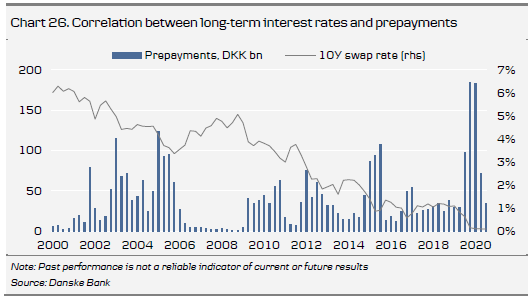
\includegraphics[width=1\linewidth]{figure/Interest_rate_and_prepayment_correlation} 

}

\caption{Pricing curve of Callabalbe Bonds and Non-callable bonds.}\label{fig:prepaymentvsswap}
\end{figure}
\hypertarget{calculating-prepayment-gains}{%
\subsection{Calculating prepayment gains}\label{calculating-prepayment-gains}}

Most Danish mortgage loans are prepaid in connection with remortgaging (debt management) or in connection with the sale of a house (though prepayment is not compulsory, as the loan may be taken over by the new owner).

The advisory services provided by banks and mortgage banks focus on the gain on the first year's net payments and on the net present value of the old loan and the new loan alternative.

Today, borrowers focus primarily on liquidity savings in the form of lower net payments and their required gains are therefore measured mainly in terms of the difference between the first year's net payments on the existing loan and the new loan. In some cases, the first year's net payments are reduced but the gain measured in terms of the net present value of future payments is negative. This would typically be the case if the borrower chooses to raise a loan with a longer term to maturity than the old loan. Under such circumstances, some borrowers will want to refinance, while others prefer to wait until the net present value gain is positive and above a threshold level.

The second parameter in the advisory service is the difference in net present values, also called the prepayment gain

The calculation of the prepayment gain is very sensitive to the yield curve applied. In practice, a flat yield curve corresponding to the after-tax yield on the refinancing alternative is often applied. The prepayment gain can be calculated using the following formula.

\[
\text { Prepayment gain }=\frac{\text { NPV }(\text { old loan })-(\text { rem. debt }+\text { costs }) \cdot \text { Disc }}{N P V(\text { old loan })}
\]
NPV (old loan) is the net present value of the old loan, corresponding to the remaining after-tax payments discounted at the after-tax yield of the new refinancing alternative. The rem. debt is the remaining debt to be refinanced and costs are the refinancing costs. Disc is the discounting factor from the payment date to the actual date on which the borrower decides to prepay the loan (no later than the notification date).

The borrower will most often be advised to refinance the mortgage based on a financial gain calculated in percent (as shown above) but also in absolute value.

\hypertarget{different-types-of-remortgaging-strategies}{%
\subsection{Different types of remortgaging strategies}\label{different-types-of-remortgaging-strategies}}

Borrowers have gradually become more conscious of managing their debt and increasingly use different remortgaging strategies to optimise their home financing.

Their choice of remortgaging strategy is heavily dependent on interest rate movements since the existing loan was raised and, in certain cases, the borrower's expectations with regard to future changes in interest rates. Below we set out a brief description of the most commonly used remortgaging strategies.

Following a substantial decline in interest rates, borrowers will benefit from remortgaging an existing loan to a new loan with a lower nominal rate of interest, as described above. The borrower will receive a gain in the form of lower future net payments and thus lower first-year net payments due to the lower interest rate. However, this type of remortgaging typically results in an increase in outstanding debt, depending on the price of the bonds underlying the new loan.

Following substantial increases in long-term interest rates, the borrower is able to reduce the outstanding debt by redeeming the old loan at a low market price and refinancing it through new bonds at a higher coupon than that of the original loan. However, this type of remortgaging leads to rising future payments because of the higher interest payments. Such remortgaging is therefore profitable only if interest rates decline again within a short time period. Borrowers initially achieve a reduction in their outstanding debt at the expense of higher payments, which they hope to be able to reduce by remortgaging to a lower coupon later.

The introduction of interest-reset loans (see Chapter 5) formed the basis of a new type of remortgaging strategy. In periods of rising long-term interest rates and a substantial steepening of the yield curve and in periods of plunging short-term interest rates, borrowers holding a loan funded by long-term fixed rate bonds may remortgage their loans by redeeming the loan and refinancing it by raising a loan based on short-term bonds. The gain achieved from adopting this strategy is a reduction in the outstanding debt and lower future mortgage payments, assuming that future short-term refinancing rates remain low. In the opposite case, where long-term interest rates have plummeted and short-term interest rates are higher than long-term interest rates, the borrower is able to reduce his mortgage payments by remortgaging from an interest-reset loan based on short-term bonds to a fixed interest rate loan based on long-term bonds.

Following the introduction of interest-reset loans, borrowers have greater opportunities for achieving future remortgaging gains because redemption of the existing loan and disbursement of the new loan may take place at interest rates across the yield curve.

\hypertarget{remortgage-gain-depends-on-several-factors}{%
\subsection{Remortgage gain depends on several factors}\label{remortgage-gain-depends-on-several-factors}}

The remortgaging gain generally depends on several debtor-specific factors. Hence, it is of significance whether the borrower is a private individual or a corporate borrower because the tax deduction rate for interest paid by the borrower varies. However, in recent years, the tax deduction rate for private borrowers has been gradually.

In `The Whitsun Package,' which was part of the 1998 tax reform, the tax deduction rate for private individuals was reduced from an average of 46\% to 33\% and in the most recent tax reform, `Forårspakken 2.0' from February 2009, the tax deduction rate was reduced yet again from 33\% to 25\% over a transitional period from 2012 to 2019. The deductible rate for businesses has also been reduced in recent years and stands at 22\% today, compared with 34\% in 1998.

Moreover, the size of the remaining principal typically determines the remortgaging gain. If the remaining principal is small, the refinancing costs in the form of a fixed fee weigh more. The gain is therefore relatively smaller than for a large remaining principal.

Finally, the remortgaging gain may depend on the term to maturity. Hence, the achieved gain is typically greater when refinancing a 30-year loan than when financing a shorter -term loan.

In recent years, greater attention in the media and campaigns launched by mortgage banks have resulted in borrowers responding more quickly to the opportunities for a remortgaging gain.

Advisory services have also become more sophisticated and borrowers are able to have their refinancing opportunities monitored, meaning they are contacted when the remortgaging gain exceeds a pre-agreed level.

\hypertarget{estimating-prepayments}{%
\section{Estimating prepayments}\label{estimating-prepayments}}

Estimating prepayments is essential to the pricing of callable covered bonds --- not just for the coming payment date but also for all future payment dates. Prepayments are important to investors as they affect cash flows. As a result, the duration of callable bonds is affected by changes in the estimated prepayment rates.

There are several different models for estimating prepayments, one of the most commonly used being the so-called capital gain requirement model where the parameters of the model are estimated based on historical prepayment data. This model assumes that a given debtor will refinance his loan if the obtainable remortgaging gain is greater than his debtor-specific required gain. Furthermore, the model allows for different debtor patterns by assuming that the various groups in the debtor distribution behave differently when it comes to borrowers' inclination to refinance at various rates. Before 1 January 2016, Danske Bank also used such a model to estimate the risk of callable bonds. In the section Danske Bank's old model for callable bonds (traditional model), we have described our old model, which in many ways is similar to other banks' models for callable bonds.

Instead of using a traditional method/model to estimate future levels of prepayments for callable bonds, Danske Bank has chosen a new path. Our new model approach is not to estimate future prepayments based on historical prepayments data (as we did before with the traditional model), but to estimate the prepayments implied by the market. Hence, this is a new and unique method to calculate the risk of callable bonds.

\hypertarget{data-for-estimating-prepayments}{%
\subsection{Data for estimating prepayments}\label{data-for-estimating-prepayments}}

One of the most important factors affecting a borrower's prepayment decision is the gain from refinancing as described in Chapter 7. Historical prepayment rates and debtor distributions are used in the estimation of the parameters in traditional capital gain requirement models (traditional models).

Historical prepayment rates for each series give a first impression of the remortgaging sensitivity of a bond series. Traditionally, series that have experienced significant prepayments can be characterised as `having lost their prepayment potential' as the remaining borrowers have presumably been able to realise decent refinancing gains at an earlier date. However, we increasingly see so-called burned-out series continuing to experience high prepayment rates.

The debtor distribution of a bond series is a breakdown of the total underlying remaining debt. A debtor distribution table breaks down loans into five groups according to the size of the remaining debt in DKKm, the share of cash and bond loans and the share of corporate and private loans. This type of distribution makes it possible to divide borrowers into 20 debtor groups.

In traditional models, large corporate loans are generally assumed to have a higher remortgaging rate than small private loans, because these loans, due to the higher remaining principal, have a lower percentage cost when prepaying. The size of the remaining principal is important due to both its relation to fixed remortgaging costs and the psychological factor that makes a gain of DKK100,000 more tempting than a gain of DKK1,000.
\begin{figure}

{\centering \includegraphics[width=1\linewidth]{figure/prepay} 

}

\caption{Pricing curve of Callabalbe Bonds and Non-callable bonds.}\label{fig:prepay}
\end{figure}
\begin{figure}

{\centering 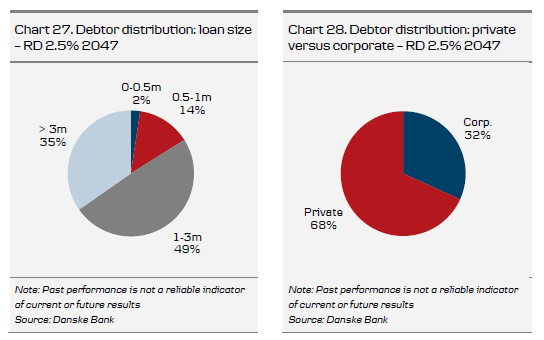
\includegraphics[width=1\linewidth]{figure/Debtor distribution} 

}

\caption{Pricing curve of Callabalbe Bonds and Non-callable bonds.}\label{fig:debitor}
\end{figure}
Every week, the individual mortgage banks publish preliminary prepayments for each
series for future, non-published payment dates. These prepayments allow for an estimation of the volume of prepayments for the next payment date (comparison with previous payment dates). They also allow for a calculation of the share of total prepayments for a given announced preliminary prepayment by using prepayment data at the same time prior to the previous payment date. The preliminary prepayment rates are used in Danske Bank's new model (SuperFly) and in the old model (Danske Analytics).

Typically, preliminary prepayments are characterised by a strong exponential increase up to expiry of the notification period. Any expectation based on announced prepayments therefore becomes more reliable as the expiry of the notification period approaches. One may also track any differences between the institutions up to the notification date.
\begin{figure}

{\centering 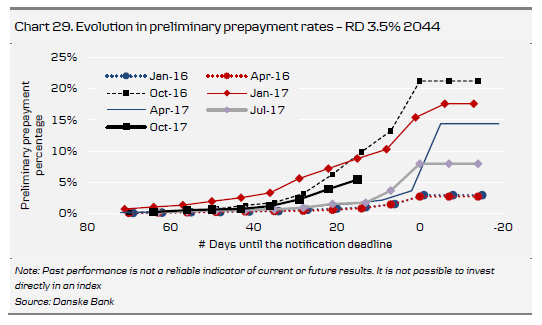
\includegraphics[width=1\linewidth]{figure/evolution in prepayments} 

}

\caption{Pricing curve of Callabalbe Bonds and Non-callable bonds.}\label{fig:PrepaymentRates}
\end{figure}
\hypertarget{term-strucutre}{%
\chapter{Term strucutre}\label{term-strucutre}}

In the classic Black-Scholes-Merton model (1973) {[}9{]} the variable of interest was the price
of a stock; a tangible and measurable quantity. Pricing and hedging was an easy task,
since the model had only one source of risk. When introducing stochastic volatility, as
done for example in the models by Heston (1993) {[}28{]} or Hagan et. al.~(2002) {[}20{]}, a side
effect was the incomplete market arising as a consequence of volatility itself not being a
traded asset. By assuming the existence of a market for derivatives, it was possible to
hedge the volatility risk of one derivative by use of another. The term structure theory
will seem somewhat similar. Assuming a market for fixed income securities depending on
a stochastic short rate, we will likewise be able to hedge one fixed income security with
another. We will start the section out by defining the short rate.

\hypertarget{the-short-rate}{%
\section{The Short Rate}\label{the-short-rate}}

We will assume the existence of a locally risk-free short rate, \(r(t)\), which follows a onefactor diffusion model. That is, given the probability space \((\Omega, \mathcal{F}, \mathbb{P})\), where \(\Omega\) is a state space, \(\mathcal{F}\) is a \(\sigma\)-algebra and \(\mathbb{P}\) is a probability measure, the short rate follows a diffusion of the form:
\[
\begin{aligned}
\mathrm{d} r_{t} &=\alpha\left(t, r_{t}\right) \mathrm{d} t+\beta\left(t, r_{t}\right) \mathrm{d} W_{t}^{\mathbb{P}} \\
r_{0} &=\bar{r}_{0}
\end{aligned}
\]
where \(W^{\mathbb{P}}=\left(W_{t}^{\mathbb{P}}\right)_{t \geq 0}\) is a standard Brownian motion under the probability measure \(\mathbb{P}\). We are explicit about the measure \(\mathbb{P}\) since we will be changing it later. We will let \(\left(\mathcal{F}_{t}\right)_{t \geq 0}\) be the information-filtration generated by \(\left(W_{t}^{\mathbb{P}}\right)_{t \geq 0}\). That the short rate is locally risk-free means that during an infinitesimal time period \([t, t+\mathrm{d} t]\), net deposits of size \(A_{t}\) will earn \(\mathrm{d} A_{t}=r_{t} A_{t} \mathrm{~d} t\) when placed in the risk-free rate. Hence, over a time interval \([t, T]\) we will have that \(A_{t}\) will grow into \(A_{T}\) given by
\[
A_{T}=A_{t} \mathrm{e}^{\int_{t}^{T} r_{s} \mathrm{~d} s}
\]
From this general representation of the risk-free rate, we will now turn to the most simple fixed income product; the zero coupon bond.

\hypertarget{zero-coupon-bonds}{%
\section{Zero Coupon Bonds}\label{zero-coupon-bonds}}

A zero coupon bond is a bond that promises the holder one unit of currency at maturity. We will make the assumption that these zero coupon bonds trade in the market. This assumption is not that hard to justify since we will often be able to replicate the zero coupon bond's payoff by static arbitrage arguments. We will further assume that the time- \(t\) price, \(P_{t}^{T}\), of a zero coupon bond maturing at time \(T\) will at most depend on the current time, the maturity and the short rate, i.e.~\(P_{t}^{T}\) is given by some function \(P\left(t, r_{t}, T\right)\). If we interpret the bond as a derivative written on the short rate, then by use of standard arbitrage arguments we have the following theorem:

Theorem 2.1. (The Term Structure PDE) The price function, \(P_{t}^{T}\), for a zero coupon bond maturing at time \(T\) must satisfy the following partial differential equation:
\(\frac{\partial P_{t}^{T}}{\partial t}+\left(\alpha\left(t, r_{t}\right)-q_{t} \beta\left(t, r_{t}\right)\right) \frac{\partial P_{t}^{T}}{\partial r}\) with terminal condition \(P_{T}^{T}=1\)
with terminal condition \(P_{T}^{T}=1\). Proof. If we are willing to assume that \(P_{t}^{T}=P\left(t, r_{t}, T\right)\) is twice continuously differentiable in \(r_{t}\) and once continuously differentiable in \(t\) then we may apply Ito's lemma get
\[
\begin{aligned}
\mathrm{d} P^{T}\left(t, r_{t}\right) &=\left(\frac{\partial P^{T}}{\partial t}+\alpha\left(t, r_{t}\right) \frac{\partial P^{T}}{\partial r}+\frac{1}{2} \beta^{2}\left(t, r_{t}\right) \frac{\partial^{2} P^{T}}{\partial r^{2}}\right) \mathrm{d} t+\beta\left(t, r_{t}\right) \frac{\partial P^{T}}{\partial r} \mathrm{dW}_{t}^{\mathbb{P}} \\
&=\alpha^{T}\left(t, r_{t}\right) P_{t}^{T} \mathrm{~d} t+\beta^{T}\left(t, r_{t}\right) P_{t}^{T} \mathrm{~d} W_{t}^{\mathbb{P}}
\end{aligned}
\]
\[ \mathrm{d} P^{T}\left(t, r_{t}\right)=\left(\frac{\partial P^{T}}{\partial t}+\alpha\left(t, r_{t}\right) \frac{\partial P^{T}}{\partial r}+\frac{1}{2} \beta^{2}\left(t, r_{t}\right) \frac{\partial^{2} P^{T}}{\partial r^{2}}\right) \mathrm{d} t+\beta\left(t, r_{t}\right) \frac{\partial P^{T}}{\partial r} \mathrm{~d} W_{t}^{\mathbb{P}} \] \(\quad=\alpha^{T}\left(t, r_{t}\right) P_{t}^{T} \mathrm{~d} t+\beta^{T}\left(t, r_{t}\right) P_{t}^{T} \mathrm{~d} W_{t}^{\mathbb{P}}\) where \[ \alpha^{T}\left(t, r_{t}\right)=\frac{\frac{\partial P^{T}}{\theta t}+\alpha\left(t, r_{t}\right) \frac{\partial P^{T}}{\theta r}+\frac{1}{2} \beta^{2}\left(t, r_{t}\right) \frac{\partial^{2} P^{T}}{\theta r^{2}}}{P_{t}^{T}} \text { and } \beta^{T}\left(t, r_{t}\right)=\frac{\beta\left(t, r_{t}\right) \frac{\partial P^{T}}{\theta r}}{P_{t}^{T}} \]
We will now establish a self-financing portfolio \(V_{t}\) of \(h_{t}^{T}\) zero coupon bonds maturing at time \(T\) and \(h_{t}^{S}\) zero coupon bonds maturing at time \(S\), i.e.~\(V_{t}\) satisfies
\[
\begin{aligned}
V_{t} &=h_{t}^{T} P_{t}^{T}+h_{t}^{S} P_{t}^{S} \\
\mathrm{~d} V_{t} &=h_{t}^{T} \mathrm{~d} P_{t}^{T}+h_{t}^{S} \mathrm{~d} P_{t}^{S}
\end{aligned}
\]
The portfolio will therefore have the following dynamics
\[
\begin{aligned}
\mathrm{d} V_{t} &=\left(h_{t}^{T} \alpha^{T}\left(t, r_{t}\right) P_{t}^{T}+h_{t}^{S} \alpha^{S}\left(t, r_{t}\right) P_{t}^{S}\right) \mathrm{d} t \\
&+\left(h_{t}^{T} \beta^{T}\left(t, r_{t}\right) P_{t}^{T}+h_{t}^{S} \beta^{S}\left(t, r_{t}\right) P_{t}^{S}\right) \mathrm{d} W_{t}^{\mathbb{P}}
\end{aligned}
\]
The idea is now to choose the portfolio in such a way that the stochastic term vanishes. Doing so leaves us with two equations in two unknowns:
\[
\begin{array}{r}
h_{t}^{T} \beta^{T}\left(t, r_{t}\right) P_{t}^{T}+h_{t}^{S} \beta^{S}\left(t, r_{t}\right) P_{t}^{S}=0 \\
h_{t}^{T} P_{t}^{T}+h_{t}^{S} P_{t}^{S}=V_{t}
\end{array}
\]

where the second equations stems from the self-financing condition. By inserting the second equation in the first yields
\[
h_{t}^{T} \beta^{T}\left(t, r_{t}\right) P_{t}^{T}+\frac{V_{t}-h_{t}^{T} P_{t}^{T}}{P_{t}^{S}} \beta^{S}\left(t, r_{t}\right) P_{t}^{S}=0 .
\]
Solving for \(h_{t}^{T}\) gives
\[
h_{t}^{T}=\frac{V_{t} \beta^{S}\left(t, r_{t}\right)}{\left(\beta^{S}\left(r, r_{t}\right)-\beta^{T}\left(r, r_{t}\right)\right) P_{t}^{T}}
\]
and by using (2.12) we also have
\[
h_{t}^{S}=-\frac{V_{t} \beta^{T}\left(t, r_{t}\right)}{\left(\beta^{S}\left(r, r_{t}\right)-\beta^{T}\left(r, r_{t}\right)\right) P_{t}^{S}} .
\]
By selecting exactly this portfolio composition, we have made the stochastic part of (2.10) vanish. Hence, the portfolio has become locally risk free, and for there to be no arbitrage, the portfolio must earn the locally risk free rate. We therefore have
\[
\left(h_{t}^{T} \alpha^{T}\left(t, r_{t}\right) P_{t}^{T}+h_{t}^{S} \alpha^{S}\left(t, r_{t}\right) P_{t}^{S}\right) \mathrm{d} t=r_{t} V_{t} \mathrm{~d} t .
\]
Inserting the portfolio holdings and simplifying we get
\[
\left(\frac{\beta^{S}\left(t, r_{t}\right) \alpha^{T}\left(t, r_{t}\right)}{\beta^{S}\left(t, r_{t}\right)-\beta^{T}\left(t, r_{t}\right)}-\frac{\beta^{T}\left(t, r_{t}\right) \alpha^{S}\left(t, r_{t}\right)}{\beta^{S}\left(t, r_{t}\right)-\beta^{T}\left(t, r_{t}\right)}\right) \mathrm{d} t=r_{t} \mathrm{~d} t .
\]
Dropping the \(\mathrm{d} t\)-terms and rearranging we obtain
\[
\frac{\alpha^{T}\left(t, r_{t}\right)-r_{t}}{\beta^{T}\left(t, r_{t}\right)}=\frac{\alpha^{S}\left(t, r_{t}\right)-r_{t}}{\beta^{S}\left(t, r_{t}\right)} .
\]
The special thing about the relation (2.18) is that the left hand side does not depend on \(S\) and the right hand side does not depend on \(T\). Hence, the ratios must be maturity independent and we may define the ratio as a function \(q_{t}=q\left(t, r_{t}\right)\) of time and the short rate:
\[
q_{t}=\frac{\alpha^{T}\left(t, r_{t}\right)-r_{t}}{\beta^{T}\left(t, r_{t}\right)} \quad \forall \quad T>0 .
\]
\(q_{t}\) is often referred to as the market price of risk or the Sharpe ratio, as it is the excess return over the risk free rate per unit of risk. We will, nevertheless, simply regard \(q_{t}\) as a consistency relation that has to hold in the market for zero coupon bonds. By inserting the expressions for \(\alpha^{T}\left(t, r_{t}\right)\) and \(\beta^{T}\left(t, r_{t}\right)\) from (2.7) in equation (2.19) and rearranging,

we arrive at the following PDE:
\[
\frac{\partial P_{t}^{T}}{\partial t}+\left(\alpha\left(t, r_{t}\right)-q_{t} \beta\left(t, r_{t}\right)\right) \frac{\partial P_{t}^{T}}{\partial r}+\frac{1}{2} \beta^{2}\left(t, r_{t}\right) \frac{\partial^{2} P_{t}^{T}}{\partial r^{2}}=r_{t} P_{t}^{T}, \quad\left(t, r_{t}\right) \in[0 ; T) \times \mathbb{R}
\]
Since the zero coupon bond matures at time \(T\) with value 1 , we may add the terminal condition \(P_{T}^{T}=1\).

Theorem \(2.1\) gives us the price of any zero coupon bond in terms of a PDE. However, we cannot simply solve the PDE since we do not know the explicit formulation of \(q_{t}\). We can deal with this problem in two ways. The first way is to assume some structure for \(q_{t}\) in which case we are implicitly making an assumption about the aggregate risk profile in the market for bonds. The second way is to assume that a market already exist and then imply \(q_{t}\) from the market prices. As we will see later, this corresponds to stating the short rate dynamics under a market consistent probability measure.

The solution to the PDE in theorem \(2.1\) can be found in different ways, but we will now introduce one particular way. Due to the Feynman-Kac theorem, we can give the price function \(P_{t}^{T}\) a stochastic representation, as presented in the following theorem.
Theorem 2.2. (Feymman-Kac) Let \(P_{t}^{T}\) be a solution to the term structure PDE in (2.4), then \(P_{t}^{T}\) will have the representation
\[
P_{t}^{T}=\mathbb{E}_{t}^{\mathrm{Q}}\left[\mathrm{e}^{-\int_{t}^{T} r_{x} \mathrm{~d} s}\right]
\]
where \(Q\) is an alternative probability measure under which the short rate follows the dynamics
\[
\mathrm{d} r_{t}=\left(\alpha\left(t, r_{t}\right)-q_{t} \beta\left(t, r_{t}\right)\right) \mathrm{d} t+\beta\left(t, r_{t}\right) \mathrm{d} W_{t}^{Q}
\]
and \(W_{t}^{\mathrm{Q}}\) is a standard Browmian motion under \(Q\).
Proof. Let \(r_{t}\) follow the \(Q\) dynamics in (2.21). Now we will apply Ito's product rule to the function \(g\left(P_{t}^{T}, A_{t}\right)=\frac{P_{t}^{T}}{A_{t}}\) with \(A_{t}=\mathrm{e}^{t_{0}^{t} r_{s} \mathrm{~d} s}\) as usual.
\[
\begin{aligned}
\mathrm{d} g\left(P_{t}^{T}, A_{t}\right) &=P_{t}^{T} \mathrm{~d} \frac{1}{A_{t}}+\frac{1}{A_{t}} \mathrm{~d} P_{t}^{T}+\mathrm{d} P_{t}^{T} \mathrm{~d} \frac{1}{A_{t}} \\
&=-r_{\mathrm{t}} \frac{P_{t}^{T}}{A_{t}} \mathrm{~d} t+\frac{1}{A_{t}} \mathrm{~d} P_{t}^{T}
\end{aligned}
\]
where \(\mathrm{d} P_{t}^{T} \mathrm{~d} \frac{1}{A_{t}}=0\) since \(\mathrm{d} \frac{1}{A_{l}}\) only contains \(\mathrm{d} t\) terms. The dynamics of \(P_{t}^{T}\) are as follows
\[
\begin{aligned}
\mathrm{d} P_{t}^{T} &=\left(\frac{\partial P_{t}^{T}}{\partial t}+\left(\alpha\left(t, r_{t}\right)-q_{t} \beta\left(t, r_{t}\right)\right) \frac{\partial P_{t}^{T}}{\partial r}+\frac{1}{2} \beta\left(t, r_{t}\right) \frac{\partial^{2} P_{t}^{T}}{\partial r^{2}}\right) \mathrm{d} t+\beta\left(t, r_{t}\right) \frac{\partial P_{t}^{T}}{\partial r} \mathrm{dW}_{t}^{\mathrm{Q}} \\
&=r_{t} P_{t}^{T} \mathrm{~d} t+\beta\left(t, r_{t}\right) \frac{\partial P_{t}^{T}}{\partial r} \mathrm{dW}_{t}^{\mathrm{Q}}
\end{aligned}
\]

which follows by using the term structure PDE. The dynamics of \(g\left(P_{t}^{T}, A_{t}\right)\) become
\[
\mathrm{d} g\left(P_{t}^{T}, A_{t}\right)=\frac{\beta\left(t, r_{t}\right)}{A_{t}} \frac{\partial P_{t}^{T}}{\partial r} \mathrm{~d} W_{t}^{\mathrm{Q}}
\]
Integrating from \(t\) to \(T\) yields
\[
g\left(P_{T}^{T}, A_{T}\right)=g\left(P_{t}^{T}, A_{t}\right)+\int_{t}^{T} \frac{\beta\left(s, r_{s}\right)}{A_{s}} \frac{\partial P_{s}^{T}}{\partial r} \mathrm{~d} W_{s}^{\mathrm{Q}}
\]
Taking conditional expectations and assuming the integrand of the stochastic integral to be in \(L^{2}\) yields the result \(^{1}\).
\[
P_{t}^{T}=\mathbb{E}_{t}^{\mathbb{Q}}\left[\mathrm{e}^{-\int_{t}^{T} r_{x} \mathrm{~d} d}\right]
\]
Theorem \(2.2\) provides a very important linkage between the solution to the term structure PDE and the expected value of a random variable. If the PDE is difficult to solve, then it might be more convenient to compute the expected value analytically or by simulations.

\hypertarget{interest-rate-swaps}{%
\section{Interest Rate Swaps}\label{interest-rate-swaps}}

A heavily traded interest rate instrument is the interest rate swap. An interest rate swap is an agreement to exchange a stream of fixed rate payments against a stream of floating rate payments. The counterparty receiving the fixed rate payment is said to have entered a receiver swap while the counterparty paying the fixed rate is said to have entered a payer swap. We will denote the payment dates of the swap by \(T_{1}, T_{2}, \ldots, T_{N}\). For the receiver swap, at each time \(T_{i-1}\), the floating rate \(R\left(T_{i-1}, T_{i}\right)\) is determined and paid out at time \(T_{i}\) against receiving the fixed rate \(K\). If for example the floating rate is the \(6 \mathrm{M}\) CIBOR, then the swap will have semi-annual payments. If the floating rate is the overnight rate then the swap is referred to as an OIS (Overnight Index Swap). In Denmark the OIS rate is also called the CITA (Copenhagen Interbank Tomorrow/Next Average) rate. Swaps with CIBOR as reference rate trade with maturities up to 30 years while CITA swaps typically trade with maturities up to one year.

If we assume the reference rate to be default-free, then we can value the floating rate leg by the following model independent argument: We consider first a floating rate bond that pays \(R\left(T_{i-1}, T_{i}\right) \delta_{i}\) at each \(T_{i}\), with \(\delta_{i}=T_{i}-T_{i-1}\), and repays the notional, \(H\), at time \(T_{N}\). Immediately after the payment at time \(T_{N-1}\), the bond will effectively be a zero coupon bond with payoff \(\left(1+R\left(T_{N-1}, T_{N}\right) \delta_{i}\right) H\) at time \(T_{N}\). Since the reference rate is default-free, and by no-arbitrage, it must hold that investing an amount \(H\) at time \(T_{N-1}\)

in \(P_{T_{N-1}}^{T_{N}}\) must yield the same return as the bond. Hence, the bond must have a value of \(H\) at time \(T_{N-1}\). As the bond has a value of \(H\) at time \(T_{N-1}\), a similar argument will hold for \(T_{N-2}\). Performing this argumentation back to time \(T_{0}\), the date of the first fixing, the floating rate note will have a value of \(H\). The value of the bond at any \(t<T_{0}\) will therefore be given by \(P_{t}^{T_{0}} H\). Since the floating rate bond pays back the notional at maturity and the floating rate leg in the swap does not, the value of the floating rate leg in the swap must be \(H\left(P_{t}^{T_{0}}-P_{t}^{T_{N}}\right)\). The fixed leg pays the deterministic amount \(K \delta_{i}\) at each payment date, so the value of these must be given by
\[
\sum_{i=1}^{N} P_{t}^{T_{1}} H K \delta_{i}
\]
It is customary to initiate a swap at a value of zero. This is ensured by finding the value of \(K\) that makes the value of the floating rate leg equal to the value of the fixed rate leg. We will denote this \(K\) as the par swap rate and it will be given by
\[
S\left(t, T_{0}, T_{N}\right)=\frac{P_{t}^{T_{0}}-P_{t}^{T_{N}}}{\sum_{i=1}^{N} P_{t}^{T_{i}} \delta_{i}}
\]
If \(T_{0}=t\), then we will denote the mapping \(T \mapsto S(t, t, T)\) the swap curve. Two other important curves are the zero coupon curve and the forward rate curve that we will define below.

\hypertarget{zero-rates-forward-rates-and-curve-fitting}{%
\section{Zero Rates, Forward Rates and Curve Fitting}\label{zero-rates-forward-rates-and-curve-fitting}}

If swap rates are available in the market for every maturity, then we can in principle solve for all the zero coupon bonds. Say that the prices of these zero coupon bonds are available, then we will define the zero rate \(y_{t}^{T}\) as the continuously compounded yield satisfying
\[
\bar{P}_{t}^{T}=\mathrm{e}^{-(T-t) y_{t}^{T}}
\]
or equivalently
\[
y_{t}^{T}=-\frac{1}{T-t} \ln \bar{P}_{t}^{T}
\]
where \(\bar{P}_{t}^{T}\) denotes the observed price in the market. Note that \(y_{t}^{T}\) contains the exact same amount of information as the zero coupon bonds themselves. However, yields can be more intuitive than prices since they take into account the time to maturity.

Another important interest rate is the forward rate. If for example funding is needed between two future points in time \(T\) and \(T+\Delta\) where \(\Delta>0\), then we can lock in a future interest rate by buying one zero coupon bond maturing at time \(T\) against selling \(\frac{\bar{P}_{t}^{T}}{\bar{P}_{t}^{T+\Delta}}\)

zero coupon bonds maturing at time \(T+\Delta\). The return earned per unit of time over the period \([T ; T+\Delta]\) will be given by
\[
F(t, T, T+\Delta)=\frac{1}{\Delta}\left(\frac{\bar{P}_{t}^{T}}{\bar{P}_{t}^{T+\Delta}}-1\right),
\]
which we will denote the time \(t\) forward rate for the future period \([T ; T+\Delta]\). If we let \(\Delta \rightarrow 0^{+}\)in (2.25) then we get the instantaneous forward rate \(f(t, T)\) :
\[
\begin{aligned}
f(t, T) &=\lim _{\Delta \rightarrow 0+} \frac{1}{\Delta}\left(\frac{\bar{P}_{t}^{T}}{\bar{P}_{t}^{T+\Delta}}-1\right) \\
&=\lim _{\Delta \rightarrow 0+} \frac{\bar{P}_{t}^{T}-\bar{P}_{t}^{T+\Delta}}{\Delta} \lim _{\Delta \rightarrow 0+} \frac{1}{\bar{P}_{t}^{T+\Delta}} \\
&=-\frac{\partial \bar{P}_{t}^{T}}{\partial T} \frac{1}{\bar{P}_{t}^{T}} \\
&=-\frac{\partial \ln \bar{P}_{t}^{T}}{\partial T} .
\end{aligned}
\]
In all of the above we have assumed that zero coupon bond prices are available for all maturities. In reality though, only a very few zero coupon bonds are available. For this reason we will rather be using the liquid swap market to imply zero coupon bonds and thereof the zero rates and forward rates. It is customary to impose some kind of interpolation scheme for the yield curve in order to connect the market observed yields. Hagan \& West (2006) {[}21{]} discuss a wide range of these interpolation schemes and in particular the so called Cubic Spline. Having observed a set of data point \(\left(\tau_{i}, y_{i}\right)\) for \(i \in\{1,2, \ldots, n\}\) from some mapping \(\tau \mapsto y(\tau)\) the Cubic Spline interpolates \(y\) by use of the following polynomial structure:
\[
y(\tau)=a_{i}+b_{i}\left(\tau-\tau_{i}\right)+c_{i}\left(\tau-\tau_{i}\right)^{2}+d_{i}\left(\tau-\tau_{i}\right)^{3} \quad \tau_{i} \leq \tau \leq \tau_{i+1}
\]
To ensure the Cubic Spline to pass through the observed points \(\left(\tau_{i}, y_{i}\right)\) we need \(a_{i}=\) \(y_{i}\). The Cubic Spline also ensures continuity of the function itself and its derivative by imposing the relations \(y_{i+1}=y_{i}+b_{i}\left(\tau_{i+1}-\tau_{i}\right)+c_{i}\left(\tau_{i+1}-\tau_{i}\right)^{2}+d_{i}\left(\tau_{i+1}-\tau_{i}\right)^{3}\) and \(b_{i+1}=b_{i}+c_{i}\left(\tau_{i+1}-\tau_{i}\right)+d_{i}\left(\tau_{i+1} \tau_{i}\right)^{2}\). For each \(i\), we now have three equations and four unknowns. Different possibilities are suggested to complete this system of equations and one such is the Hermite Spline which is also discussed by Hagan \& West. The Hermite Spline defines \(b_{i}\) as being the slope at \(\tau_{i}\) for the quadratic passing through the points \(\left(\tau_{i-1}, y_{i-1}\right),\left(\tau_{i}, y_{i}\right)\) and \(\left(\tau_{i+1}, y_{i+1}\right)\). The Hermite Spline therefore completes the system of equations and we can now use the scheme for interpolating zero rates. Since we do not observe the zero rates but instead the swap rates, we will have to find a way of computing zero rates from swap rates. If we rewrite the swap rate (2.22) for \(T_{0}=t\) in terms of the longest zero coupon bond, then we get
\[
P_{t}^{T_{N}}=\frac{1-S\left(t, t, T_{N}\right) \sum_{i=1}^{N-1} P_{t}^{T_{1}} \delta_{i}}{1+S\left(t, t, T_{N}\right) \delta_{N}} .
\]
By the definition of the \(T_{N}\) zero rate in equation (2.24), we find the corresponding zero rate as
\[
y_{t}^{T_{N}}=-\frac{1}{\tau_{N}} \ln \left(\frac{1-S\left(t, t, T_{N}\right) \sum_{i=1}^{N-1} P_{t}^{T_{i}} \delta_{i}}{1+S\left(t, t, T_{N}\right) \delta_{N}}\right)
\]
where \(\tau_{N}=T_{N}-t\). In order to find \(y_{t}^{T_{N}}\) from the market swap quotes, Hagan \& West suggested an algorithm where we choose an initial guess for \(y_{t}^{T_{N}}\) for each of the maturities for which we have swap quotes available. Then we will interpolate the zero yields by Hermite Spline for all maturities entering equation (2.28) through the zero coupon bonds, \(P_{t}^{T_{i}}=\mathrm{e}^{-\tau_{i} y_{l}\left(\tau_{i}\right)}\). From this set of zero rates, we will calculate a new set of zero rates through equation (2.28). Repeating this iterative procedure until the sum of absolute deviation of theoretical swap rates from market swap rates are less than 1 basis point results in a fast convergence.

When the Hermite Spline is applied to the zero rates, then we assure the zero curve to be differentiable and the forward curve to be continuous. As nothing assures the forward curve to be differentiable, we may end up with a non-smooth curve. If we combine equations (2.23) and (2.26), then we can find the forward curve as
\[
f(t, T)=\frac{\partial}{\partial \tau}(\tau y(\tau))
\]
Hagan \& West suggested to apply the Hermite Spline directly to the quantity \(\tau y(\tau)\) which results in a more smooth forward curve. In figure 2 , a set of market quotes as well as the bootstrapped zero and forward curves are presented for the method suggested by Hagan \& West. Note that the zero curve should not pass through the market quotes; only the swap rates implied by the zero curve should. The forward curve will be above the zero curve whenever the slope of the zero curve is positive as can be seen from the figure. Whenever we refer to the zero curve or forward curve in the rest of this thesis we will mean the interpolated approximations described in the above.

\hypertarget{caps-floors}{%
\section{Caps \& Floors}\label{caps-floors}}

Two important interest rate derivatives that will be of importance later are the so called caps and floors contracts. Since these products are highly sensitive towards changes in volatility, they are often used for calibration purposes. The cap is used to protect against increasing interest rates while the
floor is used to protect against falling interest rates

A typical cap contract could be specified to pay \(\delta_{i}\left(R\left(T_{i-1}, T_{i}\right)-K\right)^{+}\)at time \(T_{i}\) for \(i=1,2, \ldots, N\), where \(R\left(T_{i-1}, T_{i}\right)\) is some reference rate and \(K\) is the fixed cap rate. As can be seen from this payment structure, the cap is effectively a payer swap in which payments only take place if \(R\left(T_{i-1}, T_{i}\right)>K\). We will say that the cap contract is AtThe-Money (ATM) if the cap rate equals the par swap rate, i.e.~\(K=S\left(t, T_{0}, T_{N}\right)\). If we consider a single payment \(\delta_{i}\left(R\left(T_{i-1}, T_{i}\right)-K\right)^{+}\)from a cap, also known as a caplet, then this amount will be known at time \(T_{i-1}\) and hence its value must be \(\Pi\left(r_{T_{i-1}}\right)=\) \(P_{T_{i-1}}^{T_{i}} \delta_{i}\left(R\left(T_{i-1}, T_{i}\right)-K\right)^{+}\)at time \(T_{i-1}\). We write the value of the payment as \(\Pi\left(r_{T_{i-1}}\right)\) to denote that it only depends on the realised value of the short rate at time \(T_{i-1}\). Noting that the derivations of the term structure PDE of theorem (2.1) and the Feynman-Kac theorem (2.2) remain intact when changing the terminal condition to a function \(\Pi\left(r_{T}\right)\), we can write the value of the caplet as follows
\[
\text { Caplet }_{t}^{T_{i-1}}=\mathbb{E}_{t}^{\mathrm{Q}}\left[\mathrm{e}^{-\int_{1}^{T_{i-1}} r_{x} \mathrm{~d} s} P_{T_{i-1}}^{T_{i}} \delta_{i}\left(R\left(T_{i-1}, T_{i}\right)-K\right)^{+}\right]
\]
Writing \(R\left(T_{i-1}, T_{i}\right)\) in terms of \(P_{T_{i-1}}^{T_{i}}\) we can rewrite (2.30) as follows:
\[
\text { Caplet }_{t}^{T_{i-1}}=\frac{1}{K^{*}} \mathbb{E}_{t}^{\mathrm{Q}}\left[\mathrm{e}^{-\int_{t}^{T_{i-1}} r_{x} \mathrm{~d} s} K^{*} 1\left\{K^{*}>P_{T_{i-1}}^{T_{i}}\right\}-\mathrm{e}^{-\int_{t}^{T_{i-1}} r_{x} \mathrm{~d} s} P_{T_{i-1}}^{T_{i}} 1\left\{K^{*}>P_{T_{i-1}}^{T_{i}}\right\}\right]
\]
where \(K^{*}=\frac{1}{1+5 K}\). The two terms of equation \((2.31)\) can be viewed as two separate securities with payoff functions given by \(K^{*} 1\left\{K^{*}>P_{T_{i-1}}^{T_{i}}\right\}\) and \(1\left\{K^{*}>P_{T_{i-1}}^{T_{i}}\right\} P_{T_{i-1}}^{T_{i}}\)

respectively. In order to value each of these two it will make sense to make a change of measure. Consider first the price function, \(F_{t}^{T}\), of an interest rate dependent derivative expiring at time \(T\) and let \(P_{t}^{T}\) denote the time \(t\) price of a zero coupon bond maturing at time \(T\). By Ito's lemma we can find the process followed by the quantity \(F_{t}^{T} / P_{t}^{T}\) to be
\[
\mathrm{d} \frac{F_{t}^{T}}{P_{t}^{T}}=\left[\left(\beta^{T}\left(t, r_{t}\right)\right)^{2}-\beta^{T}\left(t, r_{t}\right) \beta^{F}\left(t, r_{t}\right)\right] \frac{F_{t}^{T}}{P_{t}^{T}} \mathrm{~d} t+\left(\beta^{F}\left(t, r_{t}\right)-\beta^{T}\left(t, r_{t}\right)\right) \frac{F_{t}^{T}}{P_{t}^{T}} \mathrm{~d} W_{t}^{\mathrm{Q}},
\]
where we have used that both \(F_{t}^{T}\) and \(P_{t}^{T}\) have drift \(r_{t}\) under \(\mathbb{Q}\) and \(\beta^{F}\left(t, r_{t}\right)\) indicates the volatility of \(F_{t}^{T}\). Assuming \(\beta^{T}\left(t, r_{t}\right)\) to be an adapted process then the Girsanov theorem tells us that we may define a new probability measure \(\mathbb{Q}^{T}\) through the following Radon-Nikodym derivative:
\[
\frac{\mathrm{dQ}^{T}}{\mathrm{dQ}}=\mathrm{e}^{\int_{0}^{T} \beta^{T}\left(t, r_{t}\right) d W_{t}^{Q}-\frac{1}{2}\left(\beta^{T}\left(t, r_{t}\right)\right)^{2} \mathrm{~d} t}
\]
Under this new measure we will have that
\[
W_{t}^{Q^{T}}=W_{t}^{Q}-\int_{0}^{t} \beta^{T}\left(s, r_{s}\right) \mathrm{d} s
\]
defines a Brownian motion under \(\mathbb{Q}^{T}\). The Girsanov theorem may be found in e.g.~Björk \((2009)[31]\). Inserting \((2.34)\) in \((2.32)\) we obtain
\[
\mathrm{d} \frac{F_{t}^{T}}{P_{t}^{T}}=\left(\beta^{F}\left(t, r_{t}\right)-\beta^{T}\left(t, r_{t}\right)\right) \frac{F_{t}^{T}}{P_{t}^{T}} \mathrm{~d} W_{t}^{\mathrm{Q}^{T}}
\]
From equation (2.35) we now see that the quantity \(F_{t}^{T} / P_{t}^{T}\) has no drift under \(\mathbb{Q}^{T}\). Hence, \(F_{t}^{T} / P_{t}^{T}\) must be a martingale under the \(Q^{T}\) measure and we may establish the following relation
\[
F_{t}^{T}=P_{t}^{T} \mathbb{E}_{t}^{\mathrm{Q}^{T}}\left[\frac{F_{T}^{T}}{P_{T}^{T}}\right]=P_{t}^{T} \mathbb{E}_{t}^{\mathrm{Q}^{T}}\left[F_{T}^{T}\right]
\]
where \(P_{t}^{T}\) is often called the numeraire asset. Using this technique for the first term in the expectation of (2.31) with \(P_{t}^{T_{i-1}}\) as numeraire, we find
\[
\begin{aligned}
\mathbb{E}_{t}^{\mathbb{Q}}\left[\mathrm{e}^{-\int_{t}^{T_{i-1}} r_{x} \mathrm{~d} s} K^{*} 1\left\{K^{*}>P_{T_{i-1}}^{T_{i}}\right\}\right] &=P_{t}^{T_{i-1}} K^{*} \mathbb{E}_{t}^{\mathrm{Q}^{T_{i-1}}}\left[1\left\{K^{*}>P_{T_{i-1}}^{T_{i}}\right\}\right] \\
&=P_{t^{2-1}}^{T_{i}} K^{*} \mathbb{Q}_{t}^{T_{i-1}}\left(K^{*}>P_{T_{i-1}}^{T_{i}}\right)
\end{aligned}
\]

For the second term it will be convenient to use \(P_{t}^{T_{i}}\) as a numeraire asset. Doing so and the second term of (2.31) may be written as follows
\[
\begin{aligned}
\mathbb{E}_{t}^{Q}\left[\mathrm{e}^{-\int_{t}^{T_{i-1}} r_{x} \mathrm{~d} s} 1\left\{K^{*}>P_{T_{i-1}}^{T_{i}}\right\} P_{T_{i-1}}^{T_{i}}\right] &=P_{t}^{T_{i}} \mathbb{E}_{t}^{Q^{T_{i}}}\left[\frac{1\left\{K^{*}>P_{T_{i-1}}^{T_{i}}\right\} P_{T_{i-1}}^{T_{i}}}{P_{T_{i}-1}^{T_{i}}}\right] \\
&=P_{t}^{T_{i}} \mathbb{Q}_{t}^{T_{i}}\left(K^{*}>P_{T_{i-1}}^{T_{i}}\right)
\end{aligned}
\]
Bringing the two terms back together, we find the price of the caplet to be
\[
\text { Caplet }_{t}^{T_{i-1}}=\frac{1}{K^{*}}\left[P_{t}^{T_{i-1}} K^{*} \mathbb{Q}_{t}^{T_{i-1}}\left(K^{*}>P_{T_{i-1}}^{T_{i}}\right)-P_{t}^{T_{1}} \mathbb{Q}_{t}^{T_{1}}\left(K^{*}>P_{T_{i-1}}^{T_{i}}\right)\right]
\]
Equation (2.39) has a very nice representation since we can determine the price of the caplet by calculating two probabilities under two seperate measures. The Girsanov theorem provides a linkage between these measures through equation \((2.34)\), and by using this relation, we may find the relevant short rate dynamics to be used when calculating the probabilities as
\[
\mathrm{d} r=\left(\alpha\left(t, r_{t}\right)-q_{t} \beta\left(t, r_{t}\right)+\beta\left(t, r_{t}\right) \beta^{T}\left(t, r_{t}\right)\right) \mathrm{d} t+\beta\left(t, r_{t}\right) \mathrm{d} W_{t}^{\mathrm{Q}^{T}}, \quad T \in\left\{T_{i-1}, T_{i}\right\}
\]
When we have calculated the probabilities to be used, then all there is left to do is to sum up all the caplets to get the price of the cap. The price of the cap with maturity \(T_{N}\) becomes
\[
\operatorname{Cap}_{t}^{T_{N}}=\frac{1}{K^{*}} \sum_{i=1}^{N} P_{t}^{T_{i-1}} K^{*} \mathbb{Q}_{t}^{T_{i-1}}\left(K^{*}>P_{T_{i-1}}^{T_{i}}\right)-P_{t}^{T} \mathbb{Q}_{t}^{T_{i}}\left(K^{*}>P_{T_{i-1}}^{T_{i}}\right)
\]
The probabilities in (2.41) will be model dependent, so we must return to the computation of these when we have specified a short rate model. The corresponding floor contract simply pays \(\delta\left(K-R\left(T_{i-1}, T_{i}\right)\right)^{+}\)instead of \(\delta\left(R\left(T_{i-1}, T_{i}\right)-K\right)^{+}\). Going long one cap and short one floor with same strike must therefore pay \(R\left(T_{i-1}, T_{i}\right)-K\), which is exactly the payment of a payer swap. Hence, we can price the interest rate floor by parity.

The interest rate curves and derivatives we have now defined will constitute our market, which we will assume to be available for the rest of the thesis. With our market in place, we can now turn to the callable mortgage bond.

\hypertarget{callable-mortgage-bonds}{%
\chapter{Callable Mortgage Bonds}\label{callable-mortgage-bonds}}

In this section we will look into the properties of the callable mortgage bond and build a model suited for the Danish market. Our baseline model will be the one suggested by Stanton (1995) {[}24{]}, who applied the model to the US market. Since 1995, interest rates have found their way into the negative territory, meaning that we will have to make some necessary adjustments to the model later on. For the fixed rate callable mortgage bond, the borrower will commit himself to deliver some agreed stream of payments. This payment stream could for example be defined through an annuity type loan, possibly including periods of deferred amortisation. The borrower will also hold the option to terminate the payments at any given time against paying the remaining principal. Hence, effectively the borrower is short one non-callable bond and long one call option on the bond with strike equal to the remaining principal. In contrast to usual option theory, borrowers are assumed to be faced with some barriers preventing them from prepaying as it becomes optimal. These barriers will be described in the following.

\hypertarget{callability}{%
\section{Callability}\label{callability}}

Since the borrower is effectively short one non-callable bond and long one call option, we may write the value of the mortgage liabilities to the borrower as follows
\[
M_{t}^{\ell}=B_{t}^{T}+V_{t}^{\ell}
\]
where \(B_{t}^{T}\) is the value of the non-callable bond and \(V_{t}^{\ell}\) the value of the call option as seen from the borrower. When calling the option the borrower will be faced with a fee of size \(X\) per unit of remaining principal, \(F_{t}\), where \(X\) may vary across borrowers. Think of \(X\) as the monetary costs associated with prepaying but also the non-monetary or implicit costs. If the borrower has to take time off from work in order to go to the bank, then this could be an example of an implicit cost held by the borrower. The strike value of the option therefore becomes \((1+X) F_{t}\). The value of the mortgage bond as seen from the investors point of view will be given by
\[
M_{t}^{a}=B_{t}^{T}+V_{t}^{a}
\]
\(M_{t}^{\ell}\) and \(M_{t}^{a}\) differ as the holder of the mortgage bond does not receive the costs, \(X\), associated with prepayment. If the mortgage liabilities are greater than the remaining principal plus prepayment costs, i.e.~\(M_{t}^{\ell}>(1+X) F_{t}\), then it will be optimal to prepay the mortgage. Given that it is optimal to prepay the mortgage loan, we will assume that there is a given probability that the borrower will perform a prepayment over a given period of time. That borrowers will only prepay with a certain probability when

it becomes optimal, may simply be ascribed to the fact that they cannot be expected to monitor the financial market continuously. Hence, we will assume that borrowers check for optimal prepayment at discrete points in time.

\hypertarget{prepayment-1}{%
\section{Prepayment}\label{prepayment-1}}

We will assume that the time at which a borrower checks for optimal prepayment is a stochastic event. Let \(\tau \in \mathbb{R}_{+}\)denote the next time the borrower checks for optimal prepayment, and let \(F(t)=\mathbb{P}(\tau<t)\) be the associated density. Then the so called hazard rate \(\lambda_{t}\), defined by
\[
\lambda_{t}=\lim _{h \rightarrow 0^{+}} \frac{1}{h} \mathbb{P}(t \leq \tau<t+h \mid \tau \geq t)
\]
will fully describe the probability of checking for optimal prepayment. To see this we rewrite (3.3) as follows
\[
\lambda_{t}=\lim _{h \rightarrow 0^{+}} \frac{1}{h} \frac{\mathbb{P}(\tau<t+h)-\mathbb{P}(\tau<t)}{\mathbb{P}(\tau>t)}=\lim _{h \rightarrow 0^{+}} \frac{F(t+h)-F(t)}{(1-F(t)) h}=\frac{\frac{\mathrm{d} F(t)}{\mathrm{dt}}}{1-F(t)},
\]
which can be solved for \(F\) as \(F(t)=1-\mathrm{e}^{-\int_{0}^{t} \lambda_{x} \mathrm{~d} s}\). We see that an increasing \(\lambda_{t}\) increases the probability of checking for optimal prepayment. It could be justified that \(\lambda_{t}\) should be a function of one or more market variables, but Stanton simply assumes that the intensity parameter can be in two possible states. Specifically, \(\lambda_{t}\) is defined as follows:
\[
\lambda_{t}= \begin{cases}\lambda_{1} & \text { if } M_{t}^{\ell}<\left(1+X_{i}\right) F_{t} \\ \lambda_{1}+\lambda_{2} & \text { if } M_{t}^{\ell} \geq\left(1+X_{i}\right) F_{t}\end{cases}
\]
where \(\lambda_{1}, \lambda_{2} \geq 0\) are constants. That is, if it is not optimal to prepay, i.e.~\(M_{t}^{\ell}<\left(1+X_{i}\right) F_{t}\), then a prepayment will happen according to some baseline prepayment rate \(\lambda_{1}\). If it is optimal to prepay, i.e.~\(M_{t}^{\ell} \geq\left(1+X_{i}\right) F_{t}\), then \(\lambda_{t}\) will be increased to \(\lambda_{1}+\lambda_{2}\). The reason for this split is due to the way prepayments work in the US. In the US, borrowers cannot buy back their mortgage bond in the market if the price goes below par. Nevertheless, there might be exogenous reasons making it necessary for borrowers to prepay their loan before maturity. Since these suboptimal prepayments will expectedly happen less frequently compared to the optimal prepayments, it makes sense to assume different states of the intensity parameter \(\lambda_{t}\). It is important to note, that the positive probability of investors receiving back their money at par, when the bond trades below, is a feature of the US market. In Denmark, borrowers may buy back the bonds linked to their loans, which provide them with an extra optionality to be discussed later.

\hypertarget{the-mortgage-pde}{%
\section{The Mortgage PDE}\label{the-mortgage-pde}}

We will now derive a PDE for the mortgage bond and the mortgage liabilities. As we have introduced a new source of risk through prepayments, we cannot simply let the value of a callable mortgage bond depend only on time and the short rate, as was the case for the zero coupon bond. In fact, we will have to let the price depend on both time, the short rate and some new prepayment variable, \(y_{t} .\) We will define the prepayment variable \(y_{t}\) to be a Poisson process with intensity parameter \(\lambda_{t}\). We will let \(y_{t}=0\) indicate that no prepayment has occurred and \(y_{t} \geq 1\) indicate that prepayment has occurred. The mortgager's obligations terminate at \(\tau=\inf \left\{t \in \mathbb{R} \mid y_{t} \geq 1\right\} .\) At the time of prepayment, the mortgage liabilities will jump from \(M_{\tau-}^{\ell}\) to \(M_{\tau+}^{\ell}=\left(1+X_{i}\right) F_{\tau}\) while the mortgage bond will jump from \(M_{\tau-}^{a}\) to \(M_{\tau+}^{a}=F_{\tau}\). In order to properly handle functions of discontinuous processes, we will have to shortly introduce a variation of Ito's lemma for jump processes. We will say that \(Y_{t}\) is a jump process if it takes the form
\[
Y_{t}=Y_{0}+\int_{0}^{t} \mu\left(s, Y_{s}\right) \mathrm{d} s+\int_{0}^{t} \sigma\left(s, Y_{s}\right) \mathrm{d} W_{s}+J_{t}
\]
where \(\mu\left(t, Y_{t}\right)\) and \(\sigma\left(t, Y_{t}\right)\) are adapted processes, \(W_{t}\) is a standard Brownian motion and \(J_{t}\) is an adapted pure jump process. That is, at the jump times \(\left\{\tau_{1}, \tau_{2}, \ldots\right\}, J_{t}\) will jump an amount \(\mathrm{d} J_{t}=J_{t}-J_{t-}\), where both jump times and jumps themselves may be stochastic. For such a jump process there exists a natural extension of Ito's formula and we refer to theorems 11.5.1 and 11.5.4 in Shreve (2004) {[}30{]} for one- and two-dimensional versions of the formula as well as proofs. In the present case, we have two dimensions as both the short rate, \(r_{t}\), and the prepayment variable, \(y_{t}\), follow stochastic processes. Hence, we are in a special case of a two-dimensional jump process which leads to the following corollary to theorem 11.5.4 in Shreve (2004).

Corollary 3.1. The price function of a security \(M_{t}\) depending on time, the short rate and the prepayment variable, i.e.~\(M_{t}=M\left(t, r_{t}, y_{t}\right)\), will satisfy
\[
\begin{aligned}
M_{\mathrm{t}}=& M_{0}+\int_{0}^{t} \frac{\partial M}{\partial t}\left(s, r_{s}, y_{s}\right) \mathrm{d} s+\int_{0}^{t} \frac{\partial M}{\partial r}\left(s, r_{s}, y_{s}\right) \mathrm{d} r_{s}+\int_{0}^{t} \frac{1}{2} \frac{\partial^{2} M}{\partial r^{2}}\left(s, r_{s}, y_{s}\right)\left(\mathrm{d} r_{s}\right)^{2} \\
&+\left[M\left(\tau, r_{\tau}, y_{\tau}\right)-M\left(\tau-, r_{\tau-}, y_{\tau-}\right)\right] 1(\tau \leq t)
\end{aligned}
\]
We see that the only difference in (3.7) from the usual Ito's lemma is the square bracket, ensuring that when \(y_{t}\) jumps then so does \(M_{t}\). If we write \(M_{t}\) on differential form and insert for \(r_{t}\) we get
\[
\mathrm{d} M_{t}=\alpha_{t}^{M} M_{t} \mathrm{~d} t+\beta_{t}^{M} M_{t} \mathrm{~d} W_{t}^{\mathrm{P}}+\left(M_{t}-M_{t-}\right) \mathrm{d} y_{t}
\]
where
\[
\alpha_{t}^{M}=\frac{\frac{\partial M}{\partial t}+\alpha\left(t, r_{t}\right) \frac{\partial M}{\partial r}+\frac{1}{2} \beta^{2}\left(t, r_{t}\right) \frac{\theta^{2} M}{\theta r^{2}}}{M_{t}} \text { and } \beta_{t}^{M}=\frac{\beta\left(t, r_{t}\right) \frac{\partial M}{\theta_{r}}}{M_{t}} .
\]
If the security is the callable mortgage bond then the value of the bond immediately after a jump will be the remaining principal, i.e.~\(M_{\tau}^{\alpha}=F_{\tau}\). Likewise, for the mortgage liabilities we will have \(M_{\tau}^{\ell}=\left(1+X_{i}\right) F_{\tau}\). Since we can now distinguish \(M_{t}\) from \(M_{t-}\) we may replace \(\left(M_{t}-M_{t-}\right) \mathrm{d} y_{t}\) with \(\left(F_{t}-M_{t}^{a}\right) \mathrm{d} y_{t}\) for the bond and \(\left(\left(1+X_{i}\right) F_{t}-M_{t}^{\ell}\right) \mathrm{d} y_{t}\) for the liability. Since the callable mortgage bond pays out dividends at a rate \(C_{t}\), the total gain from holding the security over an infinitesimal time-period must be \(\mathrm{d} M_{t}^{a}+C_{t} \mathrm{~d} t\). We would now like to hedge the interest rate risk of the callable bond by constructing a portfolio, \(V_{t}\), consisting of one callable mortgage bond and \(h_{t}^{T}=-\frac{\partial P_{1}^{T}}{\theta_{r}} / \frac{\partial M_{t}^{a}}{\partial r}\) zero coupon bonds maturing at time \(T\). Since the portfolio will pay dividends, we will assume that these are placed in the short rate. The amount placed in the short rate will be denoted \(h_{t}^{A}\). The self-financing condition becomes
\[
\begin{aligned}
V_{t} &=M_{t}^{a}+h_{t}^{T} P_{t}^{T}+h_{t}^{A} \\
\mathrm{~d} V_{t} &=\mathrm{d} M_{t}^{a}+C_{t} \mathrm{~d} t+h_{t}^{T} \mathrm{~d} P_{t}^{T}+h_{t}^{A} r_{t} \mathrm{~d} t
\end{aligned}
\]
Inserting the dynamics of the callable mortgage bond from (3.8) and the zero coupon bond from (2.6) we find the dynamics to be
\[
\mathrm{d} V_{t}=\left(\alpha_{t}^{M} M_{t}^{a}+C_{t}+h_{t}^{T} \alpha_{t}^{T} P_{t}^{T}+h_{t}^{A} r_{t}\right) \mathrm{d} t+\left(F_{t}-M_{t}^{a}\right) \mathrm{d} y_{t}
\]
Equation (3.12) looks almost risk free in the sense that we have eliminated all terms including Brownian increments. However, we are still left with the prepayment risk from \(y_{t}\), which we are not able to hedge. The problem is that we have introduced an idiosyncratic source of risk, as prepayment risk will vary across mortgage pools. Equation (3.12) is a dead end as seen from the perspective of arbitrage free pricing, as it defines a jump process with no other securities in the market depending on this exact source of risk. The same problem was encountered by Merton (1976) {[}25{]} when pricing options where the underlying stock price is discontinuous and Ingersoll (1977) {[}14{]} when pricing corporate convertible bonds. A pragmatic way of proceeding, used by both Merton and Ingersoll, is to replace \(\mathrm{d} y_{t}\) by its expected value, namely \(\mathbb{E}\left(\mathrm{d} y_{t}\right)=\lambda_{t} \mathrm{~d} t\). Stanton, on the other hand, implicitly assumes that prepayments will only occur at payment dates. This means that we can safely put \(\mathrm{d} y_{t}=0\) between payment dates. Strictly speaking, \(y_{t}\) is also no longer a Poisson process in this case. With this in mind, we will set \(\mathrm{d} y_{t}=0\), meaning that between payment dates equation (3.12) becomes
\[
\mathrm{d} V_{t}=\left(\alpha_{t}^{M} M_{t}+C_{t} \mathrm{~d} t+h_{t}^{T} \alpha_{t}^{T} P_{t}^{T}+h_{t}^{A} r_{t}\right) \mathrm{d} t
\]
Since equation (3.13) has been left without any stochastic sources it should earn the risk free rate, i.e.~\(\mathrm{d} V_{t}=r_{t} V_{t} \mathrm{~d} t\). Using this relation we get
\[
\left(\alpha_{t}^{M} M_{t}+C_{t}+h_{t}^{T} \alpha_{t}^{T} P_{t}^{T}+h_{t}^{A} r_{t}\right) \mathrm{d} t=r_{t}\left(M_{t}^{a}+h_{t}^{T} P_{t}^{T}+h_{t}^{A}\right) \mathrm{d} t
\]
From our derivations of the term structure PDE in section \(2.2\) we know, that under the alternative measure \(\mathbb{Q}\), the zero coupon bond has drift \(r_{t}\). Hence, by inserting \(\alpha_{t}^{M}\), switching to the \(\mathbb{Q}\) measure and using that \(\alpha_{t}^{T}=r_{t}\) under \(\mathbb{Q}\), equation (3.14) reduces to
\[
\frac{\partial M^{a}}{\partial t}+\left(\alpha\left(t, r_{t}\right)-q_{t} \beta\left(t, r_{t}\right)\right) \frac{\partial M^{a}}{\partial r}+\frac{1}{2} \beta^{2}\left(t, r_{t}\right) \frac{\partial^{2} M^{a}}{\partial r^{2}}+C_{t}=r_{t} M_{t}^{a}
\]
What is left now is to specify the dynamics of the short rate. Stanton chooses to use the CIR model by Cox, Ingersoll \& Ross (1985) {[}12{]}, where the short rate is assumed to have the \(\mathbb{P}\)-dynamics,
\[
\mathrm{d} r_{t}=\kappa\left(\mu-r_{t}\right) \mathrm{d} t+\sigma \sqrt{r_{t}} \mathrm{~d} W_{t}^{\mathrm{P}} .
\]
This specification fits into our general short rate dynamics from equation (2.1) with \(\alpha\left(t, r_{t}\right)=\kappa\left(\mu-r_{t}\right)\) and \(\beta\left(t, r_{t}\right)=\sigma \sqrt{r_{t}}\). Recall that the \(\mathbb{Q}\)-dynamics take the form
\[
\mathrm{d} r_{t}=\left(\alpha\left(t, r_{t}\right)-q_{t} \beta\left(t, r_{t}\right)\right) \mathrm{d} t+\beta\left(t, r_{t}\right) \mathrm{d} W_{t}^{Q} .
\]
Inserting for \(\alpha\left(t, r_{t}\right)\) and \(\beta\left(t, r_{t}\right)\), the \(\mathbb{Q}\)-dynamics of the CIR model becomes
\[
\mathrm{d} r_{t}=\left(\kappa\left(\mu-r_{t}\right)-q_{t} \sigma \sqrt{r_{t}}\right) \mathrm{d} t+\sigma \sqrt{r_{t}} \mathrm{~d} W_{t}^{\mathrm{Q}}
\]
As discussed earlier, it is now possible to either specify a structure for \(q_{t}\) or imply \(q_{t}\) from market prices. Cox, Ingersoll \& Ross chooses to specify \(q_{t}\) as being linear in \(\sqrt{r_{t}}{ }^{2}\) In this case we get
\[
\mathrm{d} r_{t}=\left(\kappa \mu-(\kappa+q) r_{t}\right) \mathrm{d} t+\sigma \sqrt{r_{t}} \mathrm{~d} W_{t}^{Q}
\]
for some constant \(q\). With this specification, the mortgage PDE (3.15) becomes
\[
\frac{\partial M^{a}}{\partial t}+\left(\kappa \mu-(\kappa+q) r_{t}\right) \frac{\partial M^{a}}{\partial r}+\frac{1}{2} \sigma^{2} r_{t} \frac{\partial^{2} M^{a}}{\partial r^{2}}+C_{t}=r_{t} M_{t}^{a}
\]
Similarly, the PDE obeyed by the mortgage liabilities will be given by
\[
\frac{\partial M^{\ell}}{\partial t}+\left(\kappa \mu-(\kappa+q) r_{t}\right) \frac{\partial M^{\ell}}{\partial r}+\frac{1}{2} \sigma^{2} r_{t} \frac{\partial^{2} M^{\ell}}{\partial r^{2}}+C_{t}=r_{t} M_{t}^{\ell}
\]
Before solving equations \((3.20)\) and (3.21), we will have to define the payments from \(C_{t}\). Typically, the size as well as the time of the mortgage bond payments are scheduled, and this payment schedule is distributed by the mortgage institution to the investor. However, since the mortgage bonds from a pool are not issued all at once, the payment schedule per unit of notional will change over time as issuance and prepayments occur. We will disregard this fact and simply consider a stylised world with annuity type payment streams. Given a yearly coupon rate \(R\), an initial principal \(F_{0}\) and a time to maturity \(T\), the annuity will pay a constant payment \(\bar{Y}\) at each payment date \(t_{i}\) where \(i \in\{1,2, \ldots, N\}\) and \(t_{N}=T\). Using that \(F_{t_{N}}=0\) we find that
\[
\bar{Y}=\frac{\widetilde{R}}{1-(1+\widetilde{R})^{-N}} F_{0}
\]
where \(\widetilde{R}=\frac{R}{n}\) is the periodic interest rate when there are \(n\) payments per year.

The principal will now amortise according to the following equation
\[
\frac{x^{2}-1}{x^{2}}
\]
Both results follow by standard calculations. Since the payments happen discretely in time, a smart choice is to set \(C_{t}\) equal to a sum of so called delta functions. Inspired by Wilmot et. al.~(1993) {[}23{]} we can define the Dirac delta function, \(\delta(x)\), as the limit of \(f(x)\) when \(\varepsilon \rightarrow 0^{+}\)where
\[
f(x)= \begin{cases}\frac{1}{2 \varepsilon} & |x| \leq \varepsilon \\ 0 & |x|>\varepsilon\end{cases}
\]
The special thing about \(f(x)\) is that \(\int_{-\infty}^{\infty} f(x) \mathrm{d} x=1\) for any \(\varepsilon>0\). Define now
\[
C_{t}=\sum_{i=1}^{N} \bar{Y} \delta\left(t-t_{i}\right)
\]
Then the accumulated payments, \(D_{t}\), will be given by
\[
D_{t}=\int_{0}^{t} C_{s} \mathrm{~d} s=\int_{0}^{t} \sum_{i=1}^{N} \bar{Y} \delta\left(s-t_{i}\right) \mathrm{d} s=\sum_{t_{i} \leq t} \bar{Y} .
\]
We know that from holding the mortgage bond, we will be receiving the gain \(\mathrm{d} M_{t}^{a}+C_{t} \mathrm{~d} t\) over each time-period \([t ; t+\mathrm{d} t]\). C \(_{t}\) will be zero everywhere except at payment dates, where \(\bar{Y}\) is paid out. As payment dates and prepayment dates coincide, we get notationally challenged and for this reason we will explain the jump in asset values in words. Over the payment date \(t_{i}\) the bond value \(M_{t_{i}-}^{a}\) will change to \(M_{t_{i}}^{a}\) if prepayment does not occur, but if prepayment occurs, then \(M_{t_{1}-}^{a}\) will drop to \(F_{t_{1}}\). In both cases the payment \(\bar{Y}\) is also delivered. Since this implies a stochastic boundary condition, Stanton makes the pragmatic assumption that \(M_{t_{1}-}^{a}\) - will be the expected value of the bond at time \(t_{i}\) plus the payment. We therefore have,
\[
M_{t_{i}-}^{a}=\left(1-\mathbb{P}\left(\tau=t_{i} \mid \tau \geq t_{i}\right)\right) M_{t_{i}}^{a}+\mathbb{P}\left(\tau=t_{i} \mid \tau \geq t_{i}\right) F_{t_{i}}+\bar{Y}
\]
Stanton assumes that the probability of prepayment at time \(t_{i}\) is given by \(\mathbb{P}\left(\tau=t_{i} \mid \tau \geq\right.\) \(\left.t_{i}\right)=1-\mathrm{e}^{-\int_{t_{i}}^{t_{i}+1} \lambda_{t} \mathrm{dt}} \approx 1-\mathrm{e}^{-\frac{1}{n} \lambda_{t_{i}}}\) as would be the probability if prepayment happened continuously. We therefore end up with the boundary condition
\[
M_{t_{\mathrm{u}}-}^{a}=\mathrm{e}^{-\frac{1}{n} \lambda_{t_{1}}} M_{t_{i}}^{a}+\left(1-\mathrm{e}^{-\frac{1}{m} \lambda_{t_{i}}}\right) F_{t_{i}}+\bar{Y} \quad \forall i
\]
Hence, we may solve the mortgage PDEs over each interval \(\left[t_{i-1}, t_{i}\right)\) with boundary conditions given by (3.28). We summarise our results in the following theorem.

Theorem 3.1. A callable mortgage bond delivering discrete payments of size \(\bar{Y}\) will satisfy the following PDEs over the half-open interval \(\left[t_{i-1}, t_{i}\right)\)
\[
\begin{aligned}
&\frac{\partial M^{a}}{\partial t}+\left(\kappa \mu-(\kappa+q) r_{t}\right) \frac{\partial M^{a}}{\partial r}+\frac{1}{2} \sigma^{2} r_{t} \frac{\partial^{2} M^{a}}{\partial r^{2}}=r_{t} M_{t}^{a}, \\
&\frac{\partial M^{\ell}}{\partial t}+\left(\kappa \mu-(\kappa+q) r_{t}\right) \frac{\partial M^{\ell}}{\partial r}+\frac{1}{2} \sigma^{2} r_{t} \frac{\partial^{2} M^{\ell}}{\partial r^{2}}=r_{t} M_{t}^{\ell},
\end{aligned}
\]
with boundary conditions given by
\[
\begin{aligned}
&M_{t_{1}-}^{a}=\mathrm{e}^{-\frac{1}{n} \lambda_{t_{i}}} M_{t_{i}}^{a}+\left(1-\mathrm{e}^{-\frac{1}{n} \lambda_{t_{2}}}\right) F_{t_{1}}+\bar{Y} \\
&M_{t_{1}-}^{\ell}=\mathrm{e}^{-\frac{1}{n} \lambda_{t_{1}}} M_{t_{1}}^{\ell}+\left(1-\mathrm{e}^{-\frac{1}{n} \lambda_{t_{i}}}\right)(1+X) F_{t_{1}}+\bar{Y}
\end{aligned}
\]
where
\[
\lambda_{t_{2}}= \begin{cases}\lambda_{1} & \text { if } M_{t_{i}}^{\ell}<(1+X) F_{t_{1}} \\ \lambda_{1}+\lambda_{2} & \text { if } M_{t_{i}}^{\ell} \geq(1+X) F_{t_{i}}\end{cases}
\]
for \(i \in\{0,1, \ldots, N\}\) and \(M_{t_{N}}^{a}=M_{t_{N}}^{\ell}=0\)
It is not obvious how we should solve for the mortgage bond in the theorem above analytically. Therefore, we will now look at how to approximate the solution.

\hypertarget{pricing-by-finite-differences}{%
\section{Pricing by Finite Differences}\label{pricing-by-finite-differences}}

The solution to the PDEs (3.64) and (3.65) can be approximated by use of so called finite difference techniques. The idea is simply to approximate the partial derivatives with difference quotients. For a function \(f=f(t, x)\) of time and space, we will discretise time as \(\left\{t_{0}, t_{1}, \ldots, t_{j}, \ldots, t_{J}\right\}=\{0, \Delta t, \ldots, j \Delta t, \ldots, T\}\) where \(\Delta t=\frac{T}{J}\), and space as \(\left\{x_{0}, x_{1}, \ldots, x_{i}, \ldots, x_{N}\right\}=\left\{x_{\min }, x_{\min }+\Delta x, \ldots, x_{\min }+i \Delta x, \ldots, x_{\max }\right\}\) where \(\Delta x=\frac{1}{N}\left(x_{\max }-\right.\) \(\left.x_{\min }\right)\). With this discretisation we will denote by \(f_{i, j}\) the function \(f\) evaluated in \(\left(t_{j}, x_{i}\right)\). The most common difference operators are now given in the following definition.

Definition 3.1. The forward, backward, central and second-order central differences of \(f(t, x)\) w.r.t. \(x\) are given by
\[
\begin{aligned}
D_{x}^{+} f_{i, j} &=\frac{f_{i+1, j}-f_{i, j}}{\Delta x} \\
D_{x}^{-} f_{i, j} &=\frac{f_{i, j}-f_{i-1, j}}{\Delta x} \\
D_{x} f_{i, j} &=\frac{f_{i+1, j}-f_{i-1, j}}{2 \Delta x}
\end{aligned}
\]

\[
D_{x x} f_{i, j}=\frac{f_{i+1, j}-2 f_{i, j}+f_{i-1, j}}{(\Delta x)^{2}}
\]
Different schemes exists applying different combinations of the above difference operators. The most common ones are the explicit, the implicit and the Crank-Nicolson schemes. The explicit scheme makes use of the backward difference for the time derivative as well as central and second order central differences for the first and second derivatives in space. The implicit scheme does the same in the space direction but makes use of a forward difference in the time direction. Finally, the Crank-Nicolson scheme averages the two methods. As shown in Seydel (2009) {[}27{]}, the error from approximating by use of the Crank-Nicolson scheme is of order \(\mathcal{O}\left(\Delta t^{2}\right)+\mathcal{O}\left(\Delta x^{2}\right)\) compared to the implicit and explicit methods, which are of first order in the time direction. The Crank-Nicolson method has therefore gained popularity, as it tends to be more stable than the other two methods. Defining \(m_{i, j}^{a}\) as the approximation to \(M_{t}^{a}\) in (3.64), the Crank-Nicolson method becomes
\[
\begin{array}{r}
\frac{1}{2}\left[D_{t}^{-} m_{i, j+1}^{a}+\hat{\mu}_{i} D_{r} m_{i, j+1}^{a}+\frac{1}{2} \hat{\sigma}_{i} D_{r r} m_{i, j+1}^{a}+D_{t}^{+} m_{i, j}^{a}+\hat{\mu}_{i} D_{r} m_{i, j}^{a}+\frac{1}{2} \hat{\sigma}_{i} D_{r r} m_{i, j}^{a}\right] \\
=\frac{1}{2}\left(r_{i, j+1} m_{i, j+1}^{a}+r_{i, j} m_{i, j}^{a}\right)
\end{array}
\]
where \(\hat{\mu}_{i}=\kappa \mu-(\kappa+q) r_{i, j}\) and \(\hat{\sigma}_{i}=\sigma^{2} r_{i, j}\). By inserting equations (3.34)-(3.37) and rearranging we can find the relation
\[
A_{i} m_{i-1, j}^{a}+B_{i} m_{i, j}^{a}+C_{i} m_{i+1, j}^{a}=-A_{i} m_{i-1, j+1}^{a}+D_{i} m_{i, j+1}^{a}-C_{i} m_{i+1, j+1}^{a},
\]
where
\[
\begin{aligned}
A_{i} &=\frac{1}{4 \Delta r} \hat{\mu}_{i}-\frac{1}{4(\Delta r)^{2}} \hat{\sigma}_{i} \\
B_{i} &=\frac{1}{\Delta t}+\frac{1}{2(\Delta r)^{2}} \hat{\sigma}_{i}+\frac{1}{2} r_{i, j} \\
C_{i} &=-\frac{1}{4 \Delta r} \hat{\mu}_{i}-\frac{1}{4(\Delta r)^{2}} \hat{\sigma}_{i} \\
D_{i} &=\frac{1}{\Delta t}-\frac{1}{2(\Delta r)^{2}} \hat{\sigma}_{i}-\frac{1}{2} r_{i, j+1}
\end{aligned}
\]
Define now the vector \(\mathbf{m}_{j}^{a}\) with elements \(\left[\mathbf{m}_{j}^{a}\right]_{i}=m_{i, j}^{a}\) for \(i=0,1, \ldots, N\). Having computed \(\mathrm{m}_{j+1}^{a}\), the equations (3.39)-(3.43) will define \(N-1\) equations with \(N+1\) unknowns when setting \(i=1,2, \ldots, N-1\). We encounter problems when \(i \in\{0, N\}\), since we get outside the grid by using the central differences. If we can come up with some boundary condition for \(i \in\{0, N\}\), or equivalently \(r \in\left\{r_{\min }, r_{\max }\right\}\), then it will be possible to complete the linear system of equations. A clever way to come up with boundary conditions is to consider the behaviour of either the function itself or its derivatives at high and low values of the short rate, as we might have additional information about the behaviour of the function at these values. If for example we assume the mortgage bond to have zero convexity for very high and low values of the short rate, then we may set the second derivative equal to zero in the PDEs (3.64) and (3.65). This will make the \(D_{r r}\) terms vanish in equation (3.38). The zero convexity can be justified since the embedded optionality will be either deep in or out of the money at these values. If also we replace \(D_{r} m_{0, j}\) with \(D_{r}^{+} m_{0, j}\) and replace \(D_{r} m_{N, j}\) with \(D_{r}^{-} m_{N, j}\), then we avoid using values outside the grid. All in all we can establish the following two equations:
\[
\begin{gathered}
B_{0} m_{0, j}^{a}+C_{0} m_{1, j}^{a}=D_{0} m_{0, j+1}^{a}-C_{0} m_{1, j+1}^{a} \\
A_{N} m_{N-1, j}^{a}+B_{N} m_{N, j}^{a}=-A_{N} m_{N-1, j+1}^{a}+D_{N} m_{N, j+1}^{a}
\end{gathered}
\]
where
\[
\begin{aligned}
&B_{0}=\frac{1}{\Delta t}+\frac{\hat{\mu}_{0}}{2 \Delta r}+\frac{1}{2} r_{0, j}, \quad C_{0}=-\frac{\hat{\mu}_{0}}{2 \Delta r}, \quad D_{0}=\frac{1}{\Delta t}-\frac{\hat{\mu}_{0}}{2 \Delta r}-\frac{1}{2} r_{0, j}, \\
&A_{N}=\frac{\hat{\mu}_{N}}{2 \Delta r}, \quad B_{N}=\frac{1}{\Delta t}-\frac{\hat{\mu}_{N}}{2 \Delta r}+\frac{1}{2} r_{N, j} \quad \text { and } \quad D_{N}=\frac{1}{\Delta t}+\frac{\hat{\mu}_{N}}{2 \Delta r}-\frac{1}{2} r_{N, j+1} .
\end{aligned}
\]
Since we now have \(N+1\) equations with \(N+1\) unknowns, we may write our system of equations on matrix form as follows
\[
\mathrm{Am}_{j}^{a}=\mathrm{Cm}_{j+1}^{a}
\]
where
\[
\mathbf{A}=\left[\begin{array}{ccccccc}
B_{0} & C_{0} & 0 & 0 & 0 & \cdots & 0 \\
A_{1} & B_{1} & C_{1} & 0 & 0 & \cdots & 0 \\
0 & A_{2} & B_{2} & C_{2} & 0 & \cdots & 0 \\
\vdots & & \ddots & \ddots & \ddots & & \vdots \\
\vdots & & & \ddots & \ddots & \ddots & \vdots \\
0 & \cdots & \cdots & 0 & A_{N-1} & B_{N-1} & C_{N-1} \\
0 & \cdots & \cdots & \cdots & 0 & A_{N} & B_{N}
\end{array}\right], \quad \mathbf{C}=\left[\begin{array}{cccccccc}
D_{0} & -C_{0} & 0 & 0 & 0 & \cdots & 0 \\
-A_{1} & D_{1} & -C_{1} & 0 & 0 & \cdots & 0 \\
0 & -A_{2} & D_{2} & -C_{2} & 0 & \cdots & 0 \\
\vdots & & \ddots & \ddots & \ddots & & \vdots \\
\vdots & & & \ddots & \ddots & \ddots & \vdots \\
0 & \cdots & \cdots & 0 & -A_{N-1} & D_{N-1} & -C_{N-1} \\
0 & \cdots & \cdots & \cdots & 0 & -A_{N} & D_{N}
\end{array}\right] .
\]
Performing a similar discretisation for \(M_{t}^{\ell}\) and we are able to solve for the bond price and mortgage liabilities iteratively. Algorithm \(3.1\) below gives a non-technical illustration of an implementation. The final thing that we have to do before using our finite difference solver is to choose the upper and lower values for \(r_{t}\). Since we are in the CIR model, and negative interest rates cannot occur, a natural lower bound will be \(r_{\min }=0\). In order to come up with an upper bound, we will use a value so high that it is likely not to occur. One such value could be three standard deviations away from the mean for a horizon equal to the time to maturity of the bond considered. With the upper and lower values in place, we have completed our pricing PDE solver.

The pricing algorithm has been implemented in Matlab and is available through appendix A.6. Figure 4 below shows the price of a 30 year \(12.5 \%\) annuity mortgage bond for varying prepayment intensities \(\lambda_{2}\) and varying initial short rates. As is evident from the graph, higher prepayment intensities are associated with lower values of the mortgage bond. Especially at low interest rate levels the bond exhibits negative convexity for sufficiently high prepayment intensities. Not only is the model capable of generating negative convexity, but also will the duration of the bond be negative whenever the slope of the price function is positive. This phenomenon is a consequence of the costs associated with prepayment, since the prepayment costs constitute a barrier to the mortgager who will defer a potential prepayment to a time of lower interest rates.

Before estimating and applying the model to the Danish market for callable mortgage bonds, we will consider some reasonable and necessary adjustments to the model. The CIR model used by Stanton has been developed at a time where very low and even negative interest rates had never occurred. Since the CIR model is only defined for positive interest rates, we will have to choose a short rate model capable of generating negative interest rates. Secondly, Stanton assumes that if a borrower, for some exogenous reason, choses to prepay when the mortgage bond trades below par, then the borrower will still have to prepay at par. In Denmark, all mortgage bonds are born with the option to deliver back the mortgage bond to the mortgage institution in case a borrower want to terminate his payment obligations. In the next two sections we will investigate the effect of these two adjustments.

\hypertarget{the-extended-vasicek-model}{%
\section{The Extended Vasicek Model}\label{the-extended-vasicek-model}}

In order to incorporate the presence of negative interest rates, we will introduce the extended Vasicek model by Hull \& White (1990) {[}13{]}. In this model the short rate dynamics are assumed to take the form:
\[
\mathrm{d} r_{t}=\kappa\left[\theta(t)-r_{t}\right] \mathrm{d} t+\sigma \mathrm{d} W_{t}^{\mathbb{P}}
\]
The model allows for a deterministic time dependent mean level, \(\theta(t)\). We will see that with this specification, it will be possible for the model to fit the initial term structure of interest rates if \(\theta(t)\) is chosen properly. In order to fit the model to market observables, our first job is to find the prices for zero coupon bonds in the model. From theorem \((2.4)\) we must have that the price of a zero coupon bond will satisfy the following PDE
\[
\frac{\partial P_{t}^{T}}{\partial t}+\kappa\left[\hat{\theta}(t)-r_{t}\right] \frac{\partial P_{t}^{T}}{\partial r}+\frac{1}{2} \sigma^{2} \frac{\partial^{2} P_{t}^{T}}{\partial r^{2}}=r_{t} P_{t}^{T}, \quad\left(t, r_{t}\right) \in[0 ; T) \times \mathbb{R}
\]
where \(\hat{\theta}(t)=\theta(t)-\frac{\sigma}{\kappa} q_{t}\). If we guess the general solution \(P_{t}^{T}=\mathrm{e}^{-A(t, T)-B(t, T) \mathrm{r}_{\mathrm{t}}}\) and insert into equation \((3.48)\), then we get
\[
\left[-A^{\prime}(t, T)-B^{\prime}(t, T) r_{t}\right] P_{t}^{T}-\kappa\left[\hat{\theta}(t)-r_{t}\right] B(t, T) P_{t}^{T}+\frac{1}{2} \sigma^{2} B^{2}(t, T) P_{t}^{T}=r_{t} P_{t}^{T}
\]
Dividing through by \(P_{t}^{T}\) and rearranging we obtain
\[
-A^{\prime}(t, T)-\kappa \hat{\theta}(t) B(t, T)+\frac{1}{2} \sigma^{2} B^{2}(t, T)-\left[1+B^{\prime}(t, T)-\kappa B(t, T)\right] r_{t}=0 .
\]
If equation (3.50) has to hold for all \(r_{t}\), and considering \(T\) as a parameter, then we must have that the following two ordinary differential equations must hold:
\[
\begin{array}{r}
\frac{\mathrm{d} A(t, T)}{\mathrm{d} t}+\kappa \hat{\theta}(t) B(t, T)-\frac{1}{2} \sigma^{2} B^{2}(t, T)=0 \\
1+\frac{\mathrm{d} B(t, T)}{\mathrm{d} t}-\kappa B(t, T)=0
\end{array}
\]
with terminal conditions \(A(T, T)=B(T, T)=0\). The solution to these ordinary differential equations can easily be shown to be
\[
\begin{aligned}
&B(t, T)=\frac{1}{\kappa}\left(1-\mathrm{e}^{-\kappa(T-t)}\right) \\
&A(t, T)=\kappa \int_{t}^{T} \hat{\theta}(s) B(s, T) \mathrm{d} s+\frac{\sigma^{2}}{4 \kappa} B^{2}(t, T)+\frac{\sigma^{2}}{2 \kappa^{2}}(B(t, T)-(T-t))
\end{aligned}
\]
see appendix A.1. If we at time zero observe zero coupon bond prices \(\bar{P}_{0}^{T}\) for each maturity \(T\), then the idea of Hull \& White was to choose the function \(\hat{\theta}(t)\) such that the model prices are consistent with the market prices. The function of \(\hat{\theta}(t)\) ensuring this property can be shown to be given by
\[
\hat{\theta}(t)=\bar{f}(0, t)+\frac{1}{\kappa} \frac{\mathrm{d} \bar{f}(0, t)}{\mathrm{d} t}+\frac{\sigma^{2}}{2 \kappa^{2}}\left(1-\mathrm{e}^{-2 \kappa t}\right)
\]
which implies that
\[
A(t, T)=-\ln \left(\frac{\bar{P}_{0}^{T}}{\bar{P}_{0}^{t}}\right)-B(t, T) \bar{f}(0, t)+\frac{\sigma^{2}}{4 \kappa} B^{2}(t, T)\left(1-\mathrm{e}^{-2 \kappa t}\right),
\]
where we assume that \(\bar{f}(0, t)\), the observed forward curve for the short rate, is differentiable. The derivations of equations (3.55) and (3.56) are extensive and for that reason also left in appendix A.2. To verify that we indeed fit the initial term structure, one can simply insert \(A(0, T)\) into the formula for \(P_{0}^{T}\) using that \(f(0,0)=r_{0}\).

At this point it is appropriate to have a discussion of what we have achieved by choosing \(\hat{\theta}(t)\) according to (3.55). If we had let \(\theta(t)\) be a constant, then we would be back in the original Vasicek model. Estimating the model parameters by maximum likelihood and agreeing on a specification of the market price of risk, we would be able to price zero coupon bonds and swaps by their closed form solutions. The problem with this approach is that the model most likely will not replicate the prices in the market. This is the reason why the literature and market practitioners have turned to the procedure of estimating model parameters by calibration. By this procedure we minimise the deviations of model prices from market prices by adjusting the model parameters. As is evident from this procedure, the model will lose its ability to describe the behaviour of the short rate, since the model parameters are not determined by any sound statistical estimation procedure. However, this might not necessarily be a problem. Instead of specifying the function \(q_{t}=q\left(t, r_{t}\right)\) which influences the drift part of the short rate process, we can take the market as given and let the market specify the drift rate used for pricing. Since we have assumed that a full term structure of interest rates is available in the market, we may simply regard \(q_{t}\), or equivalently \(\hat{\theta}(t)=\theta(t)-\frac{\sigma}{\kappa} q_{t}\), as being chosen by the market. For this reason we will not have a problem with our choice of \(\hat{\theta}(t)\), but we have to be aware that \(\hat{\theta}(t)\) is deterministic and therefore our choice of \(\hat{\theta}(t)\) today should also apply tomorrow. As discussed by Hull \& White themselves this assumption is likely to fail and the market practice is simply to respecify \(\theta(t)\) each time a new curve is available. It is hard to justify this practice from a theoretical viewpoint, and the main argument for proceeding with this practice anyway is the following: If we are able to price the most simple fixed income securities in the market accurately, then we will hopefully also be pricing the more complex products, like the callable bond, more accurately.

With our choice of \(\hat{\theta}(t)\) in place, we still need the parameters \(\kappa\) and \(\sigma\). As discussed by Hull \& White these could in principle also be functions of time, but in this thesis we will keep these as constants \(^{3}\). In reality we will often observe that interest rates exhibit stochastic volatility, which is of course in conflict with the constant volatility of our model. A pragmatic approach is therefore to imply the volatility and mean reversion from volatility dependent securities like the cap. In order to calibrate our model to the market for caps, we will need to be able to price these contracts. In the following we will show how to do so in the extended Vasicek model. Section \(2.5\) showed that the cap contract could be valued by computing the probabilities in the following valuation formula.
\[
\operatorname{Cap}_{t}^{T_{N}}=\frac{1}{K^{*}} \sum_{i=1}^{N} P_{t}^{T_{i-1}} K^{*} \mathbb{Q}_{t}^{T_{i-1}}\left(K^{*}>P_{T_{i-1}}^{T_{1}}\right)-P_{t}^{T_{1}} \mathbb{Q}_{t}^{T_{1}}\left(K^{*}>P_{T_{i-1}}^{T_{i}}\right)
\]
Since we have an explicit model now, we can find the dynamics under the \(\mathbb{Q}^{T}\) measure. Using that \(\beta^{T}\left(t, r_{t}\right)=-\sigma B(t, T)\) along with equation \((2.40)\) and the relevant dynamics of the short rate becomes
\[
\mathrm{d} r_{t}=\left[\kappa\left(\theta(t)-r_{t}\right)-\sigma^{2} B(t, T)\right] \mathrm{d} t+\sigma \mathrm{d} W_{t}^{\mathrm{Q}^{T}}
\]
To evaluate the probability of the event \(\left\{K^{*}>P_{T}^{S}\right\}\) we will use the result from appendix A.3 saying that \(r_{T}\) is Gaussian under both \(\mathbb{Q}^{T}\) and \(\mathbb{Q}^{S}\). Since \(P_{T}^{S}=\mathrm{e}^{-A(T, S)-B(T, S) r T}\)we will have that \(P_{T}^{S}\) is log-normal since \(-A(T, S)-B(T, S) r_{T}\) is simply a linear combination of a Gaussian variable. Let \(r_{T} \mid r_{t} \sim \mathcal{N}\left(\mu(t, T), \nu^{2}(t, T)\right)\), then we must have that \(\ln P_{T}^{S} \mid r_{t} \sim \mathcal{N}\left(\bar{\mu}(t, T, S), \bar{\nu}^{2}(t, T, S)\right)\) where \(\bar{\mu}(t, T, S)=-A(T, S)-B(T, S) \mu(t, T)\) and \(\bar{\nu}^{2}(t, T, S)=B^{2}(T, S) \nu^{2}(t, T) .\) For a log-normal random variable it holds that \(\mathbb{E}_{t}^{Q^{T}}\left[P_{T}^{S}\right]=\) \(\mathrm{e}^{\bar{\mu}(t, T, S)+\frac{1}{2} \bar{\nu}^{2}(t, T, S)}\) or equivalently \(\tilde{\mu}(t, T, S)=\ln \mathbb{E}_{t}^{\mathrm{Q}^{T}}\left[P_{T}^{S}\right]-\frac{1}{2} \bar{\nu}^{2}(t, T, S)\). Using this, we may compute the probability of \(\left\{K^{*}>P_{T}^{S}\right\}\) under \(\mathbb{Q}^{T}\) as follows:
\[
\begin{aligned}
\mathbb{Q}^{T}\left(K^{*}>P_{T}^{S}\right) &=\mathbb{Q}^{T}\left(\frac{\ln K^{*}-\bar{\mu}(t, T, S)}{\bar{\nu}(t, T, S)}>\frac{\ln P_{T}^{S}-\bar{\mu}(t, T, S)}{\bar{\nu}(t, T, S)}\right) \\
&=\Phi\left(\frac{\ln K^{*}-\bar{\mu}(t, T, S)}{\bar{\nu}(t, T, S)}\right) \\
&=\Phi\left(\frac{\ln \left(\frac{K^{*}}{\mathbb{E}_{t}^{0^{T}}\left[P_{T}^{S}\right]}\right)}{\bar{\nu}(t, T, S)}+\frac{1}{2} \bar{\nu}(t, T, S)\right)
\end{aligned}
\]
where \(\Phi(\cdot)\) denotes the standard normal CDF. We now recall that \(\frac{p_{T}^{S}}{P_{T}^{T}}\) is a martingale under \(\mathbb{Q}^{T}\). Using this property and inserting for \(\bar{\nu}(t, T, S)\), the above probability becomes
\[
\mathbb{Q}^{T}\left(K^{*}>P_{T}^{S}\right)=\Phi\left(\frac{\ln \left(\frac{K^{*} P_{t}^{T}}{P_{t}^{S}}\right)}{B(T, S) \nu(t, T)}+\frac{1}{2} B(T, S) \nu(t, T)\right)
\]
The variance of the short rate is derived in appendix A.3 and is given by
\[
\nu^{2}(t, T)=\frac{\sigma^{2}}{2 \kappa}\left(1-\mathrm{e}^{-2 \kappa(T-t)}\right) .
\]
By similar argumentation, we can find the probability of \(\left\{K^{*}>P_{T}^{S}\right\}\) under \(\mathbb{Q}^{S}\). The only thing that will change is the expectation in (3.58), which should now be evaluated under the \(\mathbb{Q}^{S}\)-measure. Appendix A.4 evaluates this expectations and we have that
\[
\mathbb{E}^{Q^{S}}\left[P_{T}^{S}\right]=\frac{P_{t}^{S}}{P_{t}^{T}} \mathrm{e}^{B^{2}(T, S) \nu^{2}(t, T)}
\]
By replacing the expectation operator in equation (3.58) with (3.59) we find that
\[
\mathbb{Q}^{S}\left(K^{*}>P_{T}^{S}\right)=\Phi\left(\frac{\ln \left(\frac{K^{*} P_{t}^{T}}{P_{t}^{S}}\right)}{B(T, S) \nu(t, T)}-\frac{1}{2} B(T, S) \nu(t, T)\right)
\]
We will summarise the above results in the following theorem.

Theorem 3.2. In the extended Vasicek model, the price of a cap contract is given by
\[
\operatorname{Cap}_{t}^{T_{N}}=\frac{1}{K^{*}} \sum_{i=1}^{N} P_{t}^{T_{i-1}} K^{*} \Phi\left(-d_{2, i}\right)-P_{t}^{T_{1}} \Phi\left(-d_{1, i}\right)
\]
where
\[
d_{1, i}=\frac{\ln \left(\frac{p_{t}^{T_{i}}}{K \cdot P_{t}^{T}-1}\right)}{B\left(T_{i-1}, T_{i}\right) \nu\left(t, T_{i-1}\right)}+\frac{1}{2} B\left(T_{i-1}, T_{i}\right) \nu\left(t, T_{i-1}\right)
\]
and
\[
d_{2, i}=d_{1, i}-B\left(T_{i-1}, T_{i}\right) \nu\left(t, T_{t-i}\right)
\]
Theorem \(3.2\) gives us a closed form solution to the price of an interest rate cap. The price function can be seen as a sum of put options on zero coupon bonds with strike \(K^{*}\), for which Jamshidian (1989) {[}8{]} was the first to derive a pricing formula equivalent to the above. It is now possible to calibrate the extended Vasicek model to market quotes. Since interest rate caps are not very liquid in the Danish market, we will use EURIBOR caps as a proxy. As the Danish krone is pegged to the Euro, and since EURIBOR and CIBOR rates tend to move together, we will expect the calibrated parameters to be a good approximation. Figure 5 shows an example of a calibration to Euro cap quotes on the \(1^{\text {st }}\) of June 2017 . Given that we have seven quotes and two parameters to be calibrated, the calibration does rather well. The calibrated parameters are \(\kappa=4.916 \cdot 10^{-11}\) and \(\sigma=0.699 \%\).

If we perform this calibration procedure over time, then we will end up with a time series of implied values for \(\kappa\) and \(\sigma\). Figure 6 shows the evolution of these parameters. From the figure it is clear that the parameters vary over time but do not diverge or explode. The volatility is low as would be expected for very short interest rates, but the mean reversion hits the zero floor in times of low interest rate levels. The mean reversion could in practice be allowed to become negative, but the model becomes unrealistic for negative \(\kappa\) as the short rate will be a diverging process. Hence, it would be meaningless to allow for negative values of \(\kappa\). An extremely low but positive \(\kappa\) is also not desirable since \(\kappa\) enters as a denominator in the equation for \(\hat{\theta}(t)\) in \((3.55)\) leading to an explosive behaviour of \(\hat{\theta}(t)\). This calibration problem seems to be very common, see for example Brigo \& Mercurio (2006) {[}5{]}, and is most likely an indication that our model is too simple to describe the behaviour of the cap market. A pragmatic way of proceeding will be to estimate \(\kappa\) by maximum likelihood as if we were in the classic Vasicek model and then use this \(\kappa\) instead. Appendix A.5 derives the maximum likelihood estimator, and by using the one year swap rate as a proxy for the short rate dynamics we find a \(\kappa\) of \(7.5 \%\). Performing a recalibration using this fixed \(\kappa\) results in a slightly higher implied volatility, a way more reasonable mean reversion and a non-explosive \(\hat{\theta}(t)\).

\hypertarget{the-delivery-option}{%
\section{The Delivery Option}\label{the-delivery-option}}

With the model extended to take into account the current negative interest rate environment, we remain to incorporate the so called delivery option. We will make the assumption that borrowers are never forced to prepay the remaining notional \(F_{t}\) whenever \(F_{t}>M_{t}^{a}\). In this scenario, we will allow the borrower to prepay \(M_{t}^{a}\) instead of \(F_{t}\), corresponding to the borrower buying back the bond and delivering it to the mortgage institution. In either case, the borrower will still have to pay the proportional prepayment cost of \(X\), such that the prepaid amount totals \((1+X) F_{t}\) if \(F_{t}<M_{t}^{a}\) and \((1+X) M_{t}^{a}\) if \(F_{t}>M_{t}^{a}\), or equivalently, \((1+X) \min \left(F_{t}, M_{t}^{a}\right)\). We will also collapse the prepayment intensities \(\lambda_{1}\) and \(\lambda_{2}\) into one prepayment intensity, \(\lambda\). We do so, since there is no longer reason to distinguish the two scenarios, as the mortgage owners can now prepay whenever they find it optimal. Compared to the case with no delivery option, the bond must decrease in value when introducing the delivery option, the reason being that the investor will no longer receive \(\min \left(F_{t}, M_{t}^{a}\right) \leq F_{t}\) in a prepayment event. With the new assumptions about the short rate dynamics and the delivery option, we may now modify theorem \(3.1\) as follows.

Theorem 3.3. (The extended Stanton model) A callable mortgage bond will satisfy the following PDEs over the half-open interval \(\left[t_{i-1}, t_{i}\right)\)
\[
\begin{aligned}
&\frac{\partial M^{a}}{\partial t}+\kappa\left(\hat{\theta}(t)-r_{t}\right) \frac{\partial M^{a}}{\partial r}+\frac{1}{2} \sigma^{2} \frac{\partial^{2} M^{a}}{\partial r^{2}}=r_{t} M_{t}^{a}, \\
&\frac{\partial M^{\ell}}{\partial t}+\kappa\left(\hat{\theta}(t)-r_{t}\right) \frac{\partial M^{\ell}}{\partial r}+\frac{1}{2} \sigma^{2} \frac{\partial^{2} M^{\ell}}{\partial r^{2}}=r_{t} M_{t}^{\ell},
\end{aligned}
\]
with boundary conditions given by
\[
\begin{aligned}
M_{t_{1}-}^{a} &=\mathrm{e}^{-\frac{1}{n} \lambda_{t_{i}}} M_{t_{i}}^{a}+\left(1-\mathrm{e}^{-\frac{1}{n} \lambda_{t_{2}}}\right) \min \left(F_{t_{1}}, M_{t_{i}}^{a}\right)+\bar{Y} \\
M_{t_{i}-}^{\ell} &=\mathrm{e}^{-\frac{1}{n} \lambda_{t_{i}}} M_{t_{i}}^{l}+\left(1-\mathrm{e}^{-\frac{1}{n} \lambda_{t_{4}}}\right)(1+X) \min \left(F_{t_{1}}, M_{t_{i}}^{a}\right)+\bar{Y} \\
\lambda_{t_{i}} &=\lambda 1\left\{M_{t_{i}}^{\ell} \geq(1+X) \min \left(F_{t_{1}}, M_{t_{i}}^{a}\right)\right\}
\end{aligned}
\]
for \(i \in\{1,2, \ldots, N\}\) and \(M_{t_{N}}^{a}=M_{t_{N}}^{\ell}=0\).
Comparing theorem \(3.3\) to theorem \(3.1\) it might seem that not much has changed, but from a computational viewpoint, we have become challenged. Most importantly \(\hat{\theta}(t)\) will have to be respecified each time a new swap curve is available and so will the implied volatility each time new cap quotes are available. From the finite difference implementation in section \(3.4\) we found that the matrices \(\mathrm{A}\) and \(\mathrm{B}\) in equation (3.46) were not changing over time. Hence, only a single matrix inversion of \(\mathbf{A}\) was needed, and for that reason we could keep it outside the loop of algorithm 1. Since A and B will now change over time, they will have to be computed in every each loop.

Prices from the extended Stanton model have been illustrated in figure 7 for a 30 year \(2.5 \%\) mortgage bond. From the figure it is clear how negative interest rates are no longer a problem. It can also be seen how the price of the bond decreases as the prepayment intensity increases since it becomes more likely that the borrower will prepay the bond when it becomes optimal. Finally, an increasing prepayment cost increases the price and adds negative convexity to the bond as borrowers will wait for interest rates to become lower before prepaying.

\hypertarget{estimating-prepayments-1}{%
\chapter{Estimating Prepayments}\label{estimating-prepayments-1}}

\hypertarget{the-danish-prepayment-data}{%
\section{The Danish Prepayment Data}\label{the-danish-prepayment-data}}

Before we jump into the actual estimation of the model, we will have a look at the characteristics of the data used in the estimation procedure. In contrast to the mortgage market in the USA, the Danish market consists of rather few but very large mortgage pools. The large mortgage pools are a result of the demand for high liquidity in the underlying mortgage bonds. The Danish data are by law \(^{4}\) published through the exchange and contains information on the borrower composition (CK92), preliminary prepayments (CK93), cash flows (CK94) and the final prepayments (CK95). The data is therefore very detailed and in practice, it is often seen that prepayment models are extended to take all kind of aspects of the data into account. In this thesis we will only consider the CK95 data, but one could for example extent the model to discriminate borrowers by loan size using the CK92 data. Figure 9 gives an example of the CK95 data for a \(5 \% 30\) year callable mortgage bond issued by Nykredit Realkredit. From the figure it is clear how the prepayments increase during times of falling interest rates as the mortgage liabilities increase during these periods. We also see a tendency that some borrowers are more quickly prepaying compared to others. This tendency is consistent with borrowers having different costs associated with prepaying, which will imply that interest rates can stay in a falling trend while prepayments keep occurring. In the next subsection we will look into how these prepayment rates may be estimated.

\hypertarget{conclusion}{%
\chapter*{Conclusion}\label{conclusion}}
\addcontentsline{toc}{chapter}{Conclusion}

\hypertarget{conclusion-nr-2}{%
\chapter*{Conclusion nr 2}\label{conclusion-nr-2}}
\addcontentsline{toc}{chapter}{Conclusion nr 2}

\appendix

\hypertarget{the-first-appendix}{%
\chapter{The First Appendix}\label{the-first-appendix}}

\hypertarget{vasicek-odes}{%
\section{Vasicek ODEs}\label{vasicek-odes}}

We have to find the solutions to the ODEs of equations (3.51) and (3.52). If we guess a solutions \(B(t, T)=\frac{1}{\kappa}\left(1-\mathrm{e}^{-\kappa(T-t)}\right)\) and insert into equation (3.52) we see that the ODE is satisfied
\[
1+\frac{\mathrm{d} B(t, T)}{\mathrm{d} t}-\kappa B(t, T)=1-\mathrm{e}^{-\kappa(T-t)}-\kappa \frac{1}{\kappa}\left(1-\mathrm{e}^{-\kappa(T-t)}\right)=0
\]
The boundary condition \(B(T, T)=\frac{1}{\kappa}\left(1-\mathrm{e}^{-\kappa(T-T)}\right)=0\) is also satisfied. Inserting \(B(t, T)\) into the ODE (3.51) and integrating from \(t\) to \(T\) we get
\[
A(T, T)-A(t, T)+\kappa \int_{t}^{T} \hat{\theta}(s) B(s, T) \mathrm{d} s-\frac{1}{2} \sigma^{2} \int_{t}^{T} B^{2}(s, T) \mathrm{d} s=0
\]
Using that \(A(T, T)=0\) and rearranging we get
\[
A(t, T)=\kappa \int_{t}^{T} \hat{\theta}(s) B(s, T) \mathrm{d} s-\frac{1}{2} \sigma^{2} \int_{t}^{T} B^{2}(s, T) \mathrm{d} s
\]
We now evaluate the integral over \(B^{2}(t, T)\) :
\[
\begin{aligned}
\int_{t}^{T} B^{2}(s, T) \mathrm{d} s &=\int_{t}^{T} \frac{1}{\kappa^{2}}\left(1+\mathrm{e}^{-2 \kappa(T-s)}-2 \mathrm{e}^{-\kappa(T-s)}\right) \mathrm{d} s \\
&=\frac{1}{\kappa^{2}}\left((T-t)+\frac{1}{2 \kappa}-\frac{1}{2 \kappa} \mathrm{e}^{-2 \kappa(T-t)}-\frac{2}{\kappa}+\frac{2}{\kappa} \mathrm{e}^{-\kappa(T-t)}\right) \\
&=\frac{1}{\kappa^{2}}\left((T-t)-\frac{1}{2 \kappa}\left(1+\mathrm{e}^{-2 \kappa(T-t)}-2 \mathrm{e}^{-\kappa(T-t)}\right)-B(t, T)\right) \\
&=\frac{1}{\kappa^{2}}\left((T-t)-\frac{\kappa}{2} B^{2}(t, T)-B(t, T)\right)
\end{aligned}
\]
Inserting (A.2) in (A.1) and we find the expression for \(A(t, T)\) :
\[
A(t, T)=\kappa \int_{t}^{T} \hat{\theta}(s) B(s, T) \mathrm{d} s+\frac{\sigma^{2}}{4 \kappa} B^{2}(t, T)+\frac{\sigma^{2}}{2 \kappa^{2}}(B(t, T)-(T-t))
\]

\hypertarget{fitting-the-initial-term-structure}{%
\section{Fitting the Initial Term structure}\label{fitting-the-initial-term-structure}}

We want to confirm that the function for \(\hat{\theta}(t)\) given in equation \((3.55)\) indeed fits the initial term structure. We start out by differentiating \(A(0, t)\) with the purpose of isolating \(\hat{\theta}(t):\)
\[
\frac{\mathrm{d} A(0, t)}{\mathrm{d} t}=\frac{\mathrm{d}}{\mathrm{d} t}\left(\kappa \int_{0}^{t} \hat{\theta}(s) B(s, t) \mathrm{d} s+\frac{\sigma^{2}}{4 \kappa} B^{2}(0, t)+\frac{\sigma^{2}}{2 \kappa^{2}}(B(0, t)-t)\right)
\]
\[
\begin{aligned}
&=\kappa \int_{0}^{t} \hat{\theta}(s) \mathrm{e}^{-\kappa(t-s)} \mathrm{d} s+\frac{\sigma^{2}}{2 \kappa} B(0, t) \frac{\mathrm{d} B(0, t)}{\mathrm{d} t}+\frac{\sigma^{2}}{2 \kappa^{2}} \frac{\mathrm{d} B(0, t)}{\mathrm{d} t}-\frac{\sigma^{2}}{2 \kappa^{2}} \\
&=\kappa \int_{0}^{t} \hat{\theta}(s) \mathrm{e}^{-\kappa(t-s)} \mathrm{d} s-\frac{\sigma^{2}}{2 \kappa^{2}}\left(\mathrm{e}^{-\kappa t}-\mathrm{e}^{-2 \kappa t}\right)-\frac{\sigma^{2}}{2 \kappa^{2}} \mathrm{e}^{-\kappa t}-\frac{\sigma^{2}}{2 \kappa^{2}} \\
&=\kappa \int_{0}^{t} \hat{\theta}(s) \mathrm{e}^{-\kappa(t-s)} \mathrm{d} s-\frac{\sigma^{2}}{2} B^{2}(0, t)
\end{aligned}
\]
We now find the second derivative to be
\[
\begin{aligned}
\frac{\mathrm{d}^{2} A(0, t)}{\mathrm{d} t^{2}} &=\kappa \hat{\theta}(t)-\kappa^{2} \int_{0}^{t} \hat{\theta}(s) \mathrm{e}^{-\kappa(t-s)} \mathrm{d} s-\sigma^{2} B(0, t) \mathrm{e}^{-\kappa t} \\
&=\kappa \hat{\theta}(t)-\kappa \frac{\mathrm{d} A(0, t)}{\mathrm{d} t}-\kappa \frac{\sigma^{2}}{2} B^{2}(0, t)-\sigma^{2} B(0, t) \mathrm{e}^{-\kappa t} \\
&=\kappa \hat{\theta}(t)-\kappa \frac{\mathrm{d} A(0, t)}{\mathrm{d} t}-\frac{\sigma^{2}}{2 \kappa}\left(1-\mathrm{e}^{-2 \kappa t}\right)
\end{aligned}
\]
In the above we have applied Leibnitz's rule \({ }^{8}\) stating that for a function \(f=f(x, t)\)
\[
\frac{\mathrm{d}}{\mathrm{d} x} \int_{u(x)}^{v(x)} f(x, t) \mathrm{d} t=f(x, v(x)) \frac{\mathrm{d} v(x)}{\mathrm{d} x}-f(x, u(x)) \frac{\mathrm{d} u(x)}{\mathrm{d} x}+\int_{u(x)}^{v(x)} \frac{\partial f(x, t)}{\partial x} \mathrm{~d} t
\]
We may now isolate \(\hat{\theta}(t)\) by rearranging (A.4):
\[
\hat{\theta}(t)=\frac{\mathrm{d} A(0, t)}{\mathrm{d} t}+\frac{1}{\kappa} \frac{\mathrm{d}^{2} A(0, t)}{\mathrm{d} t^{2}}+\frac{\sigma^{2}}{2 \kappa^{2}}\left(1-\mathrm{e}^{-2 \kappa t}\right) .
\]
Since we want to choose \(\hat{\theta}(t)\) such that market prices equals model prices, we must have
\[
\bar{P}_{0}^{t}=\mathrm{e}^{-A(0, t)-B(0, t) r_{0}} \Leftrightarrow A(0, t)=-\ln \bar{P}_{0}^{t}-B(0, t) r_{0}
\]
Differentiating \(A(0, t)\) once and twice we obtain
\[
\begin{aligned}
&\frac{\mathrm{d} A(0, t)}{\mathrm{d} t}=-\frac{\frac{\mathrm{d} P f}{\mathrm{dt}}}{\bar{P}_{0} t}-r_{0} \mathrm{e}^{-\kappa t}=\bar{f}(0, t)-r_{0} \mathrm{e}^{-\kappa t} \\
&\frac{\mathrm{d}^{2} A(0, t)}{\mathrm{d} t^{2}}=\frac{\mathrm{d} \bar{f}(0, t)}{\mathrm{d} t}+\kappa r_{0} \mathrm{e}^{-\kappa t}
\end{aligned}
\]
where we have to assume that the observed forward curve is differentiable. Inserting these derivatives in (A.5) we get
\[
\hat{\theta}(t)=\bar{f}(0, t)+\frac{1}{\kappa} \frac{\mathrm{d} \bar{f}(0, t)}{\mathrm{d} t}+\frac{\sigma^{2}}{2 \kappa^{2}}\left(1-\mathrm{e}^{-2 \kappa t}\right),
\]

which is exactly equation (3.55). Inserting this in the expression for \(A(t, T)\) we get
\[
\begin{aligned}
A(t, T) &=\int_{t}^{T} \bar{f}(0, s)\left(1-\mathrm{e}^{-\kappa(T-s)}\right) \mathrm{d} s+\frac{1}{\kappa} \int_{t}^{T} \frac{\mathrm{d} \bar{f}(0, s)}{\mathrm{d} t}\left(1-\mathrm{e}^{-\kappa(T-s)}\right) \mathrm{d} s \\
&+\int_{t}^{T} \frac{\sigma^{2}}{2 \kappa}\left(1-\mathrm{e}^{-2 \kappa s}\right) B(s, T) \mathrm{d} s+\frac{\sigma^{2}}{4 \kappa} B^{2}(t, T)+\frac{\sigma^{2}}{2 \kappa^{2}}(B(t, T)-(T-t)) \\
&=-\ln \left(\frac{\bar{P}_{0}^{T}}{\bar{P}_{0}^{t}}\right)-\int_{t}^{T} \bar{f}(0, s) \mathrm{e}^{-\kappa(T-s)} \mathrm{d} s+\frac{1}{\kappa}(\bar{f}(0, T)-\bar{f}(0, t)) \\
&-\frac{1}{\kappa} \int_{t}^{T} \frac{\mathrm{d} \bar{f}(0, s)}{\mathrm{d} t} \mathrm{e}^{-\kappa(T-s)} \mathrm{d} s+\int_{t}^{T} \frac{\sigma^{2}}{2 \kappa}\left(1-\mathrm{e}^{-2 \kappa s}\right) B(s, T) \mathrm{d} s+\frac{\sigma^{2}}{4 \kappa} B^{2}(t, T) \\
&+\frac{\sigma^{2}}{2 \kappa^{2}}(B(t, T)-(T-t))
\end{aligned}
\]
Using partial integration we have that
\[
\int_{t}^{T} \frac{\mathrm{d} \bar{f}(0, s)}{\mathrm{d} t} \mathrm{e}^{-\kappa(T-s)} \mathrm{d} s=\bar{f}(0, T)-\bar{f}(0, t) \mathrm{e}^{-\kappa(T-t)}-\kappa \int_{t}^{T} \bar{f}(0, s) \mathrm{e}^{-\kappa(T-s)} \mathrm{d} s .
\]
Inserting this in the expression for \(A(t, T)\) yields
\[
\begin{aligned}
A(t, T) &=-\ln \left(\frac{\bar{P}_{0}^{T}}{P_{0}^{t}}\right)-B(t, T) \bar{f}(0, t)+\int_{t}^{T} \frac{\sigma^{2}}{2 \kappa}\left(1-\mathrm{e}^{-2 \kappa s}\right) B(s, T) \mathrm{d} s+\frac{\sigma^{2}}{4 \kappa} B^{2}(t, T) \\
&+\frac{\sigma^{2}}{2 \kappa^{2}}(B(t, T)-(T-t))
\end{aligned}
\]
We will now evaluate the last integral:
\[
\begin{aligned}
\int_{t}^{T} \frac{\sigma^{2}}{2 \kappa}\left(1-\mathrm{e}^{-2 \kappa s}\right) B(s, T) \mathrm{d} s &=\frac{\sigma^{2}}{2 \kappa^{2}} \int_{t}^{T}\left(1-\mathrm{e}^{-2 \kappa s}\right)\left(1-\mathrm{e}^{-\kappa(T-s)}\right) \mathrm{d} s \\
&=\frac{\sigma^{2}}{2 \kappa^{2}} \int_{t}^{T} 1-\mathrm{e}^{-\kappa(T-s)}-\mathrm{e}^{-2 \kappa s}+\mathrm{e}^{-\kappa(T+s)} \mathrm{d} s \\
&=\frac{\sigma^{2}}{2 \kappa^{2}}\left[(T-t)-\frac{1}{\kappa}+\frac{1}{\kappa} \mathrm{e}^{-\kappa(T-t)}+\frac{1}{2 \kappa} \mathrm{e}^{-2 \kappa T}-\frac{1}{2 \kappa} \mathrm{e}^{-2 \kappa t}\right.\\
&\left.-\frac{1}{\kappa} \mathrm{e}^{-2 \kappa T}+\frac{1}{\kappa} \mathrm{e}^{-\kappa(T+t)}\right] \\
&=\frac{\sigma^{2}}{2 \kappa^{2}}\left[(T-t)-B(t, T)-\frac{1}{2 \kappa} \mathrm{e}^{-2 \kappa T}-\frac{1}{2 \kappa} \mathrm{e}^{-2 \kappa t}+\frac{1}{\kappa} \mathrm{e}^{-\kappa(T+t)}\right] \\
&=\frac{\sigma^{2}}{2 \kappa^{2}}\left[(T-t)-B(t, T)-\frac{\kappa}{2} \mathrm{e}^{-2 \kappa t} B^{2}(t, T)\right]
\end{aligned}
\]
Now we can insert into \(A(t, T)\) and the result follows:
\[
A(t, T)=-\ln \left(\frac{\bar{P}_{0}^{T}}{\bar{P}_{0}^{t}}\right)-B(t, T) \bar{f}(0, t)+\frac{\sigma^{2}}{4 \kappa} B^{2}(t, T)\left(1-\mathrm{e}^{-2 \kappa t}\right)
\]

\hypertarget{the-variance-of-the-short-rate}{%
\section{The Variance of the Short Rate}\label{the-variance-of-the-short-rate}}

We will determine the distribution of the short rate in the extended Vasicek model under the \(\mathbb{Q}^{T}\) measure. To do so we apply Ito's lemma to the quantity \(\mathrm{e}^{a t} r_{\mathrm{t}}\) :
\[
\begin{aligned}
\mathrm{d}\left(\mathrm{e}^{a t} r_{t}\right) &=a \mathrm{e}^{a t} r_{t} \mathrm{~d} t+\mathrm{e}^{a t} \mathrm{~d} r_{t} \\
&=a \mathrm{e}^{a t} r_{t} \mathrm{~d} t+\mathrm{e}^{a t}\left[\kappa\left(\hat{\theta}(t)-r_{t}\right)-\sigma^{2} B(t, T)\right] \mathrm{d} t+\mathrm{e}^{a t} \sigma \mathrm{d} W_{t}^{\mathrm{Q}^{T}}
\end{aligned}
\]
Choosing \(a=\kappa\) and integrating from \(t\) to \(T\) and we obtain
\[
\mathrm{e}^{\kappa T} r_{T}-\mathrm{e}^{\kappa t} r_{t}=\int_{t}^{T} \kappa \mathrm{e}^{\kappa s} \hat{\theta}(s)-\mathrm{e}^{\kappa s} \sigma^{2} B(s, T) \mathrm{d} s+\sigma \int_{t}^{T} \mathrm{e}^{a s} \mathrm{~d} W_{s}^{\mathrm{Q}^{T}}
\]
Moving \(\mathrm{e}^{\kappa t}\) to the right hand side and dividing by \(\mathrm{e}^{\kappa T}\) we obtain
\[
r_{T}=\mathrm{e}^{-\kappa(T-t)} r_{t}+\mathrm{e}^{-\kappa T} \int_{t}^{T} \kappa \mathrm{e}^{\kappa s} \hat{\theta}(s)-\mathrm{e}^{\kappa s} \sigma^{2} B(s, T) \mathrm{d} s+\sigma \mathrm{e}^{-\kappa T} \int_{t}^{T} \mathrm{e}^{\kappa s} \mathrm{~d} W_{s}^{\mathrm{Q}^{T}}
\]
Since \(e^{\kappa t}\) is just a deterministic function, the stochastic integral will be normally distributed. The variance of \(r_{T}\) will therefore be given by
\[
\begin{aligned}
\mathbb{V}_{t}^{\mathbb{Q}^{T}}\left[r_{T}\right] &=\mathbb{V}_{t}^{\mathbb{Q}^{T}}\left[\sigma \mathrm{e}^{-\kappa T} \int_{t}^{T} \mathrm{e}^{\kappa s} \mathrm{~d} W_{s}^{\mathbb{Q}^{T}}\right] \\
&=\sigma^{2} \mathrm{e}^{-2 \kappa T} \int_{t}^{T} \mathrm{e}^{2 \kappa s} \mathrm{~d} s \\
&=\frac{\sigma^{2}}{2 \kappa} \mathrm{e}^{-2 \kappa T}\left(\mathrm{e}^{2 \kappa T}-\mathrm{e}^{2 \kappa t}\right) \\
&=\frac{\sigma^{2}}{2 \kappa}\left(1-\mathrm{e}^{-2 \kappa(T-t)}\right)
\end{aligned}
\]

\hypertarget{the-expected-value-under-mathbbqs}{%
\section{\texorpdfstring{The Expected Value Under \(\mathbb{Q}\)\^{}S}{The Expected Value Under \textbackslash mathbb\{Q\}\^{}S}}\label{the-expected-value-under-mathbbqs}}

We would like to evaluate the expectation \(\mathbb{E}^{Q^{S}}\left[P_{T}^{S}\right]\). We know that any price process deflated by \(P_{t}^{S}\) is a martingale under \(\mathbb{Q}^{S}\) and in particular by equation (2.35) we have that
\[
\mathrm{d} \frac{P_{t}^{T}}{P_{t}^{S}}=\left(\beta^{T}\left(t, r_{t}\right)-\beta^{S}\left(t, r_{t}\right)\right) \frac{P_{t}^{T}}{P_{t}^{S}} \mathrm{~d} W_{t}^{Q^{S}}
\]
Since we are in the extended Vasicek model we have \(\beta^{T}\left(t, r_{t}\right)=-\sigma B(t, T)\) and \(\beta^{S}\left(t, r_{t}\right)=\) \(-\sigma B(t, S)\). Inserting these we get
\[
\mathrm{d} \frac{P_{t}^{T}}{P_{t}^{S}}=\sigma(B(t, S)-B(t, T)) \frac{P_{t}^{T}}{P_{t}^{S}} \mathrm{~d} W_{t}^{Q^{S}}
\]
Since \(P_{T}^{T}=1\) we must have \(\mathbb{E}^{Q^{S}}\left[P_{T}^{S}\right]=\mathbb{E}^{Q^{S}}\left[\frac{P_{T}^{S}}{P_{T}^{T}}\right]\). To evaluate this expectation we will need the distribution of \(\frac{p_{t}^{S}}{p_{t}^{X}}\). By Ito's lemma and equation (A.8) we have that
\[
\mathrm{d} \frac{P_{t}^{S}}{P_{t}^{T}}=\sigma^{2}(B(t, S)-B(t, T))^{2} \frac{P_{t}^{S}}{P_{t}^{T}} \mathrm{~d} t-\sigma(B(t, S)-B(t, T)) \frac{P_{t}^{S}}{P_{t}^{T}} \mathrm{~d} W_{t}^{Q^{S}}
\]
Taking the logarithm of \(\frac{P_{t}^{S}}{P_{t}^{T}}\) and using again Ito's lemma we get
\[
\mathrm{d} \ln \frac{P_{t}^{S}}{P_{t}^{T}}=\frac{1}{2} \sigma^{2}(B(t, S)-B(t, T))^{2} \mathrm{~d} t-\sigma(B(t, S)-B(t, T)) \mathrm{d} W_{t}^{\mathrm{Q}^{S}}
\]
Integrating from \(t\) to \(T\) and rearranging yields
\[
\frac{P_{T}^{S}}{P_{T}^{T}}=\frac{P_{t}^{S}}{P_{t}^{T}} \mathrm{e} J_{t}^{T} \frac{1}{2} \sigma^{2}(B(u, S)-B(u, T))^{2} \mathrm{~d} u-\sigma \int_{t}^{T}(B(u, S)-B(u, T)) \mathrm{d} W_{u}^{0^{S}}
\]
The inside of the exponential function will be Gaussian, so we will determine the mean \(\hat{\mu}\) and variance \(\hat{\sigma}^{2}\). The mean can be found as
\[
\begin{aligned}
\hat{\mu} &=\int_{t}^{T} \frac{1}{2} \sigma^{2}(B(u, S)-B(u, T))^{2} \mathrm{~d} u \\
&=\frac{\sigma^{2}}{2 \kappa^{2}} \int_{t}^{T}\left(\mathrm{e}^{-\kappa(T-u)}-\mathrm{e}^{-\kappa(S-u)}\right)^{2} \mathrm{~d} u \\
&=\frac{\sigma^{2}}{2 \kappa^{2}}\left(\mathrm{e}^{-\kappa T}-\mathrm{e}^{-\kappa S}\right)^{2} \int_{t}^{T} \mathrm{e}^{2 \kappa u} \mathrm{~d} u \\
&=\frac{\sigma^{2}}{4 \kappa^{3}}\left(\mathrm{e}^{-\kappa T}-\mathrm{e}^{-\kappa S}\right)^{2}\left(\mathrm{e}^{2 \kappa T}-\mathrm{e}^{2 \kappa t}\right) \\
&=\frac{\sigma^{2}}{4 \kappa^{3}} \mathrm{e}^{-2 \kappa T}\left(1-\mathrm{e}^{-\kappa(S-T)}\right)^{2}\left(\mathrm{e}^{2 \kappa T}-\mathrm{e}^{2 \kappa t}\right) \\
&=\frac{\sigma^{2}}{4 \kappa^{3}}\left(1-\mathrm{e}^{-\kappa(S-T)}\right)^{2}\left(1-\mathrm{e}^{-2 \kappa(T-t)}\right) \\
&=\frac{1}{2} B^{2}(T, S) \nu^{2}(t, T)
\end{aligned}
\]
The variance can be found as
\[
\begin{aligned}
\hat{\sigma}^{2} &=\mathbb{V}_{t}^{\mathrm{Q}^{S}}\left(-\sigma \int_{t}^{T} B(u, S)-B(u, T) \mathrm{d} W_{u}^{Q^{S}}\right) \\
&=\sigma^{2} \int_{t}^{T}(B(u, S)-B(u, T))^{2} \mathrm{~d} u \\
&=2 \hat{\mu} .
\end{aligned}
\]

Let \(X \sim \mathcal{N}\left(\hat{\mu}, \hat{\sigma}^{2}\right)\), then we can now evaluate the desired expectation:
\[
\begin{aligned}
\mathbb{E}_{t}^{Q^{S}}\left[\frac{P_{T}^{S}}{P_{T}^{T}}\right] &=\frac{P_{t}^{S}}{P_{t}^{T}} \mathbb{E}\left[\mathrm{e}^{X}\right] \\
&=\frac{P_{t}^{S}}{P_{t}^{T}} \mathrm{e}^{\tilde{\mu}+\frac{1}{2} \dot{\sigma}^{2}} \\
&=\frac{P_{t}^{S}}{P_{t}^{T}} \mathrm{e}^{B^{2}(T, S) \nu^{2}(t, T)}
\end{aligned}
\]

\hypertarget{vasicek-mle}{%
\section{Vasicek MLE}\label{vasicek-mle}}

By similar calculations as in A.3 and using that \(\theta(t)=\theta\) is a constant, we can find
\[
r_{T}=\mathrm{e}^{-\kappa(T-t)} r_{t}+\theta\left[1-\mathrm{e}^{-\kappa(T-t)}\right]+\sigma \mathrm{e}^{-\kappa T} \int_{t}^{T} \mathrm{e}^{\kappa s} \mathrm{~d} W_{s}^{\mathbb{P}}
\]
The conditional mean is given by
\[
\mathbb{E}_{t}\left[r_{T}\right]=\mathrm{e}^{-\kappa(T-t)} r_{t}+\theta\left[1-\mathrm{e}^{-\kappa(T-t)}\right]
\]
and appendix A.3 derived the variance as
\[
\mathbb{V}_{t}\left[r_{T}\right]=\frac{\sigma^{2}}{2 \kappa}\left(1-\mathrm{e}^{-2 \mathrm{k}(T-t)}\right)
\]
Since the stochastic integral is Gaussian, we will have that the increments are also Gaussian, and the conditional density will therefore be
\[
f_{r_{i_{i}}}\left(x \mid r_{t_{i-1}}, \kappa, \theta, \sigma\right)=\frac{1}{\sqrt{2 \pi \nu_{i}}} \mathrm{e}^{-\frac{\left(x-\mu_{i}\right)^{2}}{2 \nu_{i}}},
\]
where
\[
\mu_{i}=\mathrm{e}^{-\kappa \Delta t_{i} r_{t_{i-1}}}+\theta\left[1-\mathrm{e}^{-\kappa \Delta t_{i}}\right], \quad \nu_{i}=\frac{\sigma^{2}}{2 \kappa_{i}}\left(1-\mathrm{e}^{-2 \kappa \Delta t_{i}}\right) \quad \text { and } \quad \Delta t_{i}=t_{i}-t_{i-1}
\]
The log likelihood is therefore given by
\[
\log \mathcal{L}\left(\kappa, \theta, \sigma \mid\left\{r_{t_{i}}\right\}_{i=0}^{N}\right)=-\frac{N}{2} \ln (2 \pi)-\sum_{i=1}^{N} \ln v_{i}+\frac{\left(r_{t_{i}}-\mu_{i}\right)^{2}}{2 \nu_{i}^{2}}
\]
Performing an estimation in Matlab for the period 1996 to 2017 with the \(1 \mathrm{Y}\) swap rate as a proxy for the dynamics of the short rate and we get the results in table 6 .

\hypertarget{roadmap}{%
\chapter*{Roadmap}\label{roadmap}}
\addcontentsline{toc}{chapter}{Roadmap}

\hypertarget{timeline}{%
\section*{Timeline}\label{timeline}}
\addcontentsline{toc}{section}{Timeline}

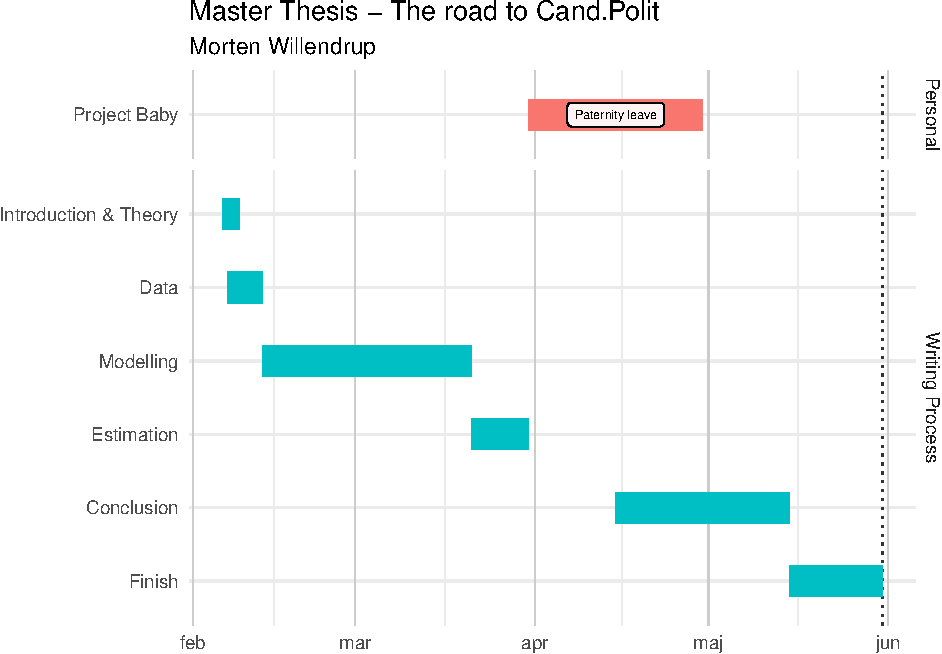
\includegraphics{thesis_files/figure-latex/roadmap-1.pdf}

\hypertarget{logbook}{%
\section*{Logbook}\label{logbook}}
\addcontentsline{toc}{section}{Logbook}

\hypertarget{introduction}{%
\subsection*{Introduction}\label{introduction}}
\addcontentsline{toc}{subsection}{Introduction}

Need to write a full introduction of the Danish Mortgage Market, furthermore
leave space for a brief walkthorugh of the thesis
\begin{itemize}
\tightlist
\item
  10/02/22 - Wrote a section on the Danish Bond market, needs some rewritining
\item
  11/02/22 - Wrote section about term structure and the danish bond market mathematically
\end{itemize}
\hypertarget{theory}{%
\subsection*{Theory}\label{theory}}
\addcontentsline{toc}{subsection}{Theory}

Relevant theory should be Machine Learning, which is relevent should be discussed
in detail

\hypertarget{data}{%
\subsection*{Data}\label{data}}
\addcontentsline{toc}{subsection}{Data}

Get data from DST.\\
Get data from Nasdaq.\\
Get data from Danske Bank Asset Management

\backmatter

\hypertarget{references}{%
\chapter*{References}\label{references}}
\addcontentsline{toc}{chapter}{References}

\markboth{References}{References}

\noindent

\setlength{\parindent}{-0.20in}

\hypertarget{refs}{}
\begin{CSLReferences}{1}{0}
\leavevmode\vadjust pre{\hypertarget{ref-dick2012corporate}{}}%
Dick-Nielsen, Jens, Peter Feldhütter, and David Lando. 2012. {``Corporate Bond Liquidity Before and After the Onset of the Subprime Crisis.''} \emph{Journal of Financial Economics} 103 (3). Elsevier: 471--92.

\leavevmode\vadjust pre{\hypertarget{ref-ECBC2021}{}}%
ECBC. 2021. {``European Covered Bond Fact Bbook 2021.''} \url{https://hypo.org/app/uploads/sites/3/2021/09/ECBC-Fact-Book-2021-FINAL.pdf}.

\leavevmode\vadjust pre{\hypertarget{ref-Gundersen2011}{}}%
Gundersen, Poul, Stig Hesselberg, and Sean Hove. 2011. {``Danish Mortgage Credit.''} \emph{Monetary Review}. Nationalbanken.

\leavevmode\vadjust pre{\hypertarget{ref-jensen2013rentesregning}{}}%
Jensen, Bjarne Astrup. 2013. \emph{Rentesregning: S{æ}rtryk Af 6. Udgave}. Dj{ø}f Forlag.

\end{CSLReferences}

% Index?

\end{document}
